% Options for packages loaded elsewhere
\PassOptionsToPackage{unicode}{hyperref}
\PassOptionsToPackage{hyphens}{url}
%
\documentclass[
]{article}
\title{models with mice}
\author{}
\date{\vspace{-2.5em}}

\usepackage{amsmath,amssymb}
\usepackage{lmodern}
\usepackage{iftex}
\ifPDFTeX
  \usepackage[T1]{fontenc}
  \usepackage[utf8]{inputenc}
  \usepackage{textcomp} % provide euro and other symbols
\else % if luatex or xetex
  \usepackage{unicode-math}
  \defaultfontfeatures{Scale=MatchLowercase}
  \defaultfontfeatures[\rmfamily]{Ligatures=TeX,Scale=1}
\fi
% Use upquote if available, for straight quotes in verbatim environments
\IfFileExists{upquote.sty}{\usepackage{upquote}}{}
\IfFileExists{microtype.sty}{% use microtype if available
  \usepackage[]{microtype}
  \UseMicrotypeSet[protrusion]{basicmath} % disable protrusion for tt fonts
}{}
\makeatletter
\@ifundefined{KOMAClassName}{% if non-KOMA class
  \IfFileExists{parskip.sty}{%
    \usepackage{parskip}
  }{% else
    \setlength{\parindent}{0pt}
    \setlength{\parskip}{6pt plus 2pt minus 1pt}}
}{% if KOMA class
  \KOMAoptions{parskip=half}}
\makeatother
\usepackage{xcolor}
\IfFileExists{xurl.sty}{\usepackage{xurl}}{} % add URL line breaks if available
\IfFileExists{bookmark.sty}{\usepackage{bookmark}}{\usepackage{hyperref}}
\hypersetup{
  pdftitle={models with mice},
  hidelinks,
  pdfcreator={LaTeX via pandoc}}
\urlstyle{same} % disable monospaced font for URLs
\usepackage[left=0.5cm,right=0.5cm,top=0.5cm,bottom=0.5cm]{geometry}
\usepackage{graphicx}
\makeatletter
\def\maxwidth{\ifdim\Gin@nat@width>\linewidth\linewidth\else\Gin@nat@width\fi}
\def\maxheight{\ifdim\Gin@nat@height>\textheight\textheight\else\Gin@nat@height\fi}
\makeatother
% Scale images if necessary, so that they will not overflow the page
% margins by default, and it is still possible to overwrite the defaults
% using explicit options in \includegraphics[width, height, ...]{}
\setkeys{Gin}{width=\maxwidth,height=\maxheight,keepaspectratio}
% Set default figure placement to htbp
\makeatletter
\def\fps@figure{htbp}
\makeatother
\setlength{\emergencystretch}{3em} % prevent overfull lines
\providecommand{\tightlist}{%
  \setlength{\itemsep}{0pt}\setlength{\parskip}{0pt}}
\setcounter{secnumdepth}{-\maxdimen} % remove section numbering
\usepackage{dcolumn}
\usepackage{array}
\usepackage{pdflscape}
\newcommand{\blandscape}{\begin{landscape}}
\newcommand{\elandscape}{\end{landscape}}
\usepackage{booktabs}
\usepackage{longtable}
\usepackage{array}
\usepackage{multirow}
\usepackage{wrapfig}
\usepackage{float}
\usepackage{colortbl}
\usepackage{pdflscape}
\usepackage{tabu}
\usepackage{threeparttable}
\usepackage{threeparttablex}
\usepackage[normalem]{ulem}
\usepackage{makecell}
\usepackage{xcolor}
\usepackage{fontspec}
\usepackage{multicol}
\usepackage{hhline}
\newlength\Oldarrayrulewidth
\newlength\Oldtabcolsep
\usepackage{hyperref}
\ifLuaTeX
  \usepackage{selnolig}  % disable illegal ligatures
\fi

\begin{document}
\maketitle

{
\setcounter{tocdepth}{2}
\tableofcontents
}
\hypertarget{bar-plot-state-x-pdevelop}{%
\section{Bar plot: STATE X PDEVELOP}\label{bar-plot-state-x-pdevelop}}

\hypertarget{barplot-of-demographics}{%
\section{barplot of demographics}\label{barplot-of-demographics}}

\hypertarget{can-do-something-with-accept-reject-and-reluctantly-accept.}{%
\section{Can do something with accept, reject and reluctantly
accept.}\label{can-do-something-with-accept-reject-and-reluctantly-accept.}}

\hypertarget{formice-dataset}{%
\section{FORMICE DATASET}\label{formice-dataset}}

\hypertarget{kahan-scale}{%
\section{Kahan scale}\label{kahan-scale}}

\hypertarget{mar-condition-and-missing-data-pattern}{%
\subsection{MAR condition and missing data
pattern}\label{mar-condition-and-missing-data-pattern}}

\hypertarget{mifa}{%
\subsection{Mifa}\label{mifa}}

\begin{landscape}
\newpage

\hypertarget{efa-pretty-table}{%
\subsection{EFA Pretty Table}\label{efa-pretty-table}}

\global\setlength{\Oldarrayrulewidth}{\arrayrulewidth}

\global\setlength{\Oldtabcolsep}{\tabcolsep}

\setlength{\tabcolsep}{0pt}

\renewcommand*{\arraystretch}{1.5}



\providecommand{\ascline}[3]{\noalign{\global\arrayrulewidth #1}\arrayrulecolor[HTML]{#2}\cline{#3}}

\begin{longtable}[c]{|p{1.00in}|p{4.50in}|p{0.75in}|p{0.75in}|p{0.75in}|p{0.75in}|p{0.75in}}

\caption{Table\ 1:\ EFA\ on\ adapted\ Cultural\ Cognition\ Scale\ from\ Kahan\ et\ al(2007)}\\

\ascline{1.5pt}{666666}{1-7}

\multicolumn{1}{>{\raggedright}m{\dimexpr 1in+0\tabcolsep}}{\textcolor[HTML]{000000}{\fontsize{10}{10}\selectfont{\global\setmainfont{Helvetica}{Code}}}} & \multicolumn{1}{>{\raggedright}m{\dimexpr 4.5in+0\tabcolsep}}{\textcolor[HTML]{000000}{\fontsize{10}{10}\selectfont{\global\setmainfont{Helvetica}{Items}}}} & \multicolumn{1}{>{\raggedright}m{\dimexpr 0.75in+0\tabcolsep}}{\textcolor[HTML]{000000}{\fontsize{10}{10}\selectfont{\global\setmainfont{Helvetica}{Egalitarianism}}}} & \multicolumn{1}{>{\raggedright}m{\dimexpr 0.75in+0\tabcolsep}}{\textcolor[HTML]{000000}{\fontsize{10}{10}\selectfont{\global\setmainfont{Helvetica}{Communitarianism}}}} & \multicolumn{1}{>{\raggedleft}m{\dimexpr 0.75in+0\tabcolsep}}{\textcolor[HTML]{000000}{\fontsize{10}{10}\selectfont{\global\setmainfont{Helvetica}{Communality}}}} & \multicolumn{1}{>{\raggedleft}m{\dimexpr 0.75in+0\tabcolsep}}{\textcolor[HTML]{000000}{\fontsize{10}{10}\selectfont{\global\setmainfont{Helvetica}{Uniqueness}}}} & \multicolumn{1}{>{\raggedleft}m{\dimexpr 0.75in+0\tabcolsep}}{\textcolor[HTML]{000000}{\fontsize{10}{10}\selectfont{\global\setmainfont{Helvetica}{Complexity}}}} \\

\ascline{1.5pt}{666666}{1-7}\endfirsthead \caption[]{Table\ 1:\ EFA\ on\ adapted\ Cultural\ Cognition\ Scale\ from\ Kahan\ et\ al(2007)}\\

\ascline{1.5pt}{666666}{1-7}

\multicolumn{1}{>{\raggedright}m{\dimexpr 1in+0\tabcolsep}}{\textcolor[HTML]{000000}{\fontsize{10}{10}\selectfont{\global\setmainfont{Helvetica}{Code}}}} & \multicolumn{1}{>{\raggedright}m{\dimexpr 4.5in+0\tabcolsep}}{\textcolor[HTML]{000000}{\fontsize{10}{10}\selectfont{\global\setmainfont{Helvetica}{Items}}}} & \multicolumn{1}{>{\raggedright}m{\dimexpr 0.75in+0\tabcolsep}}{\textcolor[HTML]{000000}{\fontsize{10}{10}\selectfont{\global\setmainfont{Helvetica}{Egalitarianism}}}} & \multicolumn{1}{>{\raggedright}m{\dimexpr 0.75in+0\tabcolsep}}{\textcolor[HTML]{000000}{\fontsize{10}{10}\selectfont{\global\setmainfont{Helvetica}{Communitarianism}}}} & \multicolumn{1}{>{\raggedleft}m{\dimexpr 0.75in+0\tabcolsep}}{\textcolor[HTML]{000000}{\fontsize{10}{10}\selectfont{\global\setmainfont{Helvetica}{Communality}}}} & \multicolumn{1}{>{\raggedleft}m{\dimexpr 0.75in+0\tabcolsep}}{\textcolor[HTML]{000000}{\fontsize{10}{10}\selectfont{\global\setmainfont{Helvetica}{Uniqueness}}}} & \multicolumn{1}{>{\raggedleft}m{\dimexpr 0.75in+0\tabcolsep}}{\textcolor[HTML]{000000}{\fontsize{10}{10}\selectfont{\global\setmainfont{Helvetica}{Complexity}}}} \\

\ascline{1.5pt}{666666}{1-7}\endhead



\multicolumn{1}{>{\raggedright}m{\dimexpr 1in+0\tabcolsep}}{\textcolor[HTML]{000000}{\fontsize{10}{10}\selectfont{\global\setmainfont{Helvetica}{K\_ERADEQ1}}}} & \multicolumn{1}{>{\raggedright}m{\dimexpr 4.5in+0\tabcolsep}}{\textcolor[HTML]{000000}{\fontsize{10}{10}\selectfont{\global\setmainfont{Helvetica}{(E)We\ need\ to\ dramatically\ reduce\ inequalities\ between\ the\ rich\ and\ the\ poor.}}}} & \multicolumn{1}{>{\raggedright}m{\dimexpr 0.75in+0\tabcolsep}}{\textcolor[HTML]{000000}{\fontsize{10}{10}\selectfont{\global\setmainfont{Helvetica}{0.653}}}} & \multicolumn{1}{>{\raggedright}m{\dimexpr 0.75in+0\tabcolsep}}{\textcolor[HTML]{000000}{\fontsize{10}{10}\selectfont{\global\setmainfont{Helvetica}{}}}} & \multicolumn{1}{>{\raggedleft}m{\dimexpr 0.75in+0\tabcolsep}}{\textcolor[HTML]{000000}{\fontsize{10}{10}\selectfont{\global\setmainfont{Helvetica}{0.427}}}} & \multicolumn{1}{>{\raggedleft}m{\dimexpr 0.75in+0\tabcolsep}}{\textcolor[HTML]{000000}{\fontsize{10}{10}\selectfont{\global\setmainfont{Helvetica}{0.573}}}} & \multicolumn{1}{>{\raggedleft}m{\dimexpr 0.75in+0\tabcolsep}}{\textcolor[HTML]{000000}{\fontsize{10}{10}\selectfont{\global\setmainfont{Helvetica}{1.002}}}} \\





\multicolumn{1}{>{\raggedright}m{\dimexpr 1in+0\tabcolsep}}{\textcolor[HTML]{000000}{\fontsize{10}{10}\selectfont{\global\setmainfont{Helvetica}{K\_ERADEQ2}}}} & \multicolumn{1}{>{\raggedright}m{\dimexpr 4.5in+0\tabcolsep}}{\textcolor[HTML]{000000}{\fontsize{10}{10}\selectfont{\global\setmainfont{Helvetica}{(E)We\ need\ to\ dramatically\ reduce\ inequalities\ between\ men\ and\ women.}}}} & \multicolumn{1}{>{\raggedright}m{\dimexpr 0.75in+0\tabcolsep}}{\textcolor[HTML]{000000}{\fontsize{10}{10}\selectfont{\global\setmainfont{Helvetica}{0.593}}}} & \multicolumn{1}{>{\raggedright}m{\dimexpr 0.75in+0\tabcolsep}}{\textcolor[HTML]{000000}{\fontsize{10}{10}\selectfont{\global\setmainfont{Helvetica}{}}}} & \multicolumn{1}{>{\raggedleft}m{\dimexpr 0.75in+0\tabcolsep}}{\textcolor[HTML]{000000}{\fontsize{10}{10}\selectfont{\global\setmainfont{Helvetica}{0.352}}}} & \multicolumn{1}{>{\raggedleft}m{\dimexpr 0.75in+0\tabcolsep}}{\textcolor[HTML]{000000}{\fontsize{10}{10}\selectfont{\global\setmainfont{Helvetica}{0.648}}}} & \multicolumn{1}{>{\raggedleft}m{\dimexpr 0.75in+0\tabcolsep}}{\textcolor[HTML]{000000}{\fontsize{10}{10}\selectfont{\global\setmainfont{Helvetica}{1.004}}}} \\





\multicolumn{1}{>{\raggedright}m{\dimexpr 1in+0\tabcolsep}}{\textcolor[HTML]{000000}{\fontsize{10}{10}\selectfont{\global\setmainfont{Helvetica}{K\_EWEALTH}}}} & \multicolumn{1}{>{\raggedright}m{\dimexpr 4.5in+0\tabcolsep}}{\textcolor[HTML]{000000}{\fontsize{10}{10}\selectfont{\global\setmainfont{Helvetica}{(E)Our\ society\ would\ be\ better\ off\ if\ the\ distribution\ of\ wealth\ was\ more\ equal.}}}} & \multicolumn{1}{>{\raggedright}m{\dimexpr 0.75in+0\tabcolsep}}{\textcolor[HTML]{000000}{\fontsize{10}{10}\selectfont{\global\setmainfont{Helvetica}{0.539}}}} & \multicolumn{1}{>{\raggedright}m{\dimexpr 0.75in+0\tabcolsep}}{\textcolor[HTML]{000000}{\fontsize{10}{10}\selectfont{\global\setmainfont{Helvetica}{}}}} & \multicolumn{1}{>{\raggedleft}m{\dimexpr 0.75in+0\tabcolsep}}{\textcolor[HTML]{000000}{\fontsize{10}{10}\selectfont{\global\setmainfont{Helvetica}{0.314}}}} & \multicolumn{1}{>{\raggedleft}m{\dimexpr 0.75in+0\tabcolsep}}{\textcolor[HTML]{000000}{\fontsize{10}{10}\selectfont{\global\setmainfont{Helvetica}{0.686}}}} & \multicolumn{1}{>{\raggedleft}m{\dimexpr 0.75in+0\tabcolsep}}{\textcolor[HTML]{000000}{\fontsize{10}{10}\selectfont{\global\setmainfont{Helvetica}{1.160}}}} \\





\multicolumn{1}{>{\raggedright}m{\dimexpr 1in+0\tabcolsep}}{\textcolor[HTML]{000000}{\fontsize{10}{10}\selectfont{\global\setmainfont{Helvetica}{K\_EDISCRIM}}}} & \multicolumn{1}{>{\raggedright}m{\dimexpr 4.5in+0\tabcolsep}}{\textcolor[HTML]{000000}{\fontsize{10}{10}\selectfont{\global\setmainfont{Helvetica}{(E)Discrimination\ against\ minorities\ is\ still\ a\ very\ serious\ problem\ in\ our\ society.}}}} & \multicolumn{1}{>{\raggedright}m{\dimexpr 0.75in+0\tabcolsep}}{\textcolor[HTML]{000000}{\fontsize{10}{10}\selectfont{\global\setmainfont{Helvetica}{0.512}}}} & \multicolumn{1}{>{\raggedright}m{\dimexpr 0.75in+0\tabcolsep}}{\textcolor[HTML]{000000}{\fontsize{10}{10}\selectfont{\global\setmainfont{Helvetica}{}}}} & \multicolumn{1}{>{\raggedleft}m{\dimexpr 0.75in+0\tabcolsep}}{\textcolor[HTML]{000000}{\fontsize{10}{10}\selectfont{\global\setmainfont{Helvetica}{0.314}}}} & \multicolumn{1}{>{\raggedleft}m{\dimexpr 0.75in+0\tabcolsep}}{\textcolor[HTML]{000000}{\fontsize{10}{10}\selectfont{\global\setmainfont{Helvetica}{0.686}}}} & \multicolumn{1}{>{\raggedleft}m{\dimexpr 0.75in+0\tabcolsep}}{\textcolor[HTML]{000000}{\fontsize{10}{10}\selectfont{\global\setmainfont{Helvetica}{1.385}}}} \\





\multicolumn{1}{>{\raggedright}m{\dimexpr 1in+0\tabcolsep}}{\textcolor[HTML]{000000}{\fontsize{10}{10}\selectfont{\global\setmainfont{Helvetica}{K\_HEQUAL}}}} & \multicolumn{1}{>{\raggedright}m{\dimexpr 4.5in+0\tabcolsep}}{\textcolor[HTML]{000000}{\fontsize{10}{10}\selectfont{\global\setmainfont{Helvetica}{(H)We\ have\ gone\ too\ far\ in\ pushing\ equal\ rights\ in\ this\ country.}}}} & \multicolumn{1}{>{\raggedright}m{\dimexpr 0.75in+0\tabcolsep}}{\textcolor[HTML]{000000}{\fontsize{10}{10}\selectfont{\global\setmainfont{Helvetica}{0.434}}}} & \multicolumn{1}{>{\raggedright}m{\dimexpr 0.75in+0\tabcolsep}}{\textcolor[HTML]{000000}{\fontsize{10}{10}\selectfont{\global\setmainfont{Helvetica}{}}}} & \multicolumn{1}{>{\raggedleft}m{\dimexpr 0.75in+0\tabcolsep}}{\textcolor[HTML]{000000}{\fontsize{10}{10}\selectfont{\global\setmainfont{Helvetica}{0.206}}}} & \multicolumn{1}{>{\raggedleft}m{\dimexpr 0.75in+0\tabcolsep}}{\textcolor[HTML]{000000}{\fontsize{10}{10}\selectfont{\global\setmainfont{Helvetica}{0.794}}}} & \multicolumn{1}{>{\raggedleft}m{\dimexpr 0.75in+0\tabcolsep}}{\textcolor[HTML]{000000}{\fontsize{10}{10}\selectfont{\global\setmainfont{Helvetica}{1.192}}}} \\





\multicolumn{1}{>{\raggedright}m{\dimexpr 1in+0\tabcolsep}}{\textcolor[HTML]{000000}{\fontsize{10}{10}\selectfont{\global\setmainfont{Helvetica}{K\_HREVDIS1}}}} & \multicolumn{1}{>{\raggedright}m{\dimexpr 4.5in+0\tabcolsep}}{\textcolor[HTML]{000000}{\fontsize{10}{10}\selectfont{\global\setmainfont{Helvetica}{(H)Nowadays\ it\ seems\ like\ there\ is\ just\ as\ much\ discrimination\ against\ upper\ castes\ as\ there\ is\ against\ Dalits.}}}} & \multicolumn{1}{>{\raggedright}m{\dimexpr 0.75in+0\tabcolsep}}{\textcolor[HTML]{000000}{\fontsize{10}{10}\selectfont{\global\setmainfont{Helvetica}{0.427}}}} & \multicolumn{1}{>{\raggedright}m{\dimexpr 0.75in+0\tabcolsep}}{\textcolor[HTML]{000000}{\fontsize{10}{10}\selectfont{\global\setmainfont{Helvetica}{}}}} & \multicolumn{1}{>{\raggedleft}m{\dimexpr 0.75in+0\tabcolsep}}{\textcolor[HTML]{000000}{\fontsize{10}{10}\selectfont{\global\setmainfont{Helvetica}{0.185}}}} & \multicolumn{1}{>{\raggedleft}m{\dimexpr 0.75in+0\tabcolsep}}{\textcolor[HTML]{000000}{\fontsize{10}{10}\selectfont{\global\setmainfont{Helvetica}{0.815}}}} & \multicolumn{1}{>{\raggedleft}m{\dimexpr 0.75in+0\tabcolsep}}{\textcolor[HTML]{000000}{\fontsize{10}{10}\selectfont{\global\setmainfont{Helvetica}{1.036}}}} \\





\multicolumn{1}{>{\raggedright}m{\dimexpr 1in+0\tabcolsep}}{\textcolor[HTML]{000000}{\fontsize{10}{10}\selectfont{\global\setmainfont{Helvetica}{K\_IINTRFER}}}} & \multicolumn{1}{>{\raggedright}m{\dimexpr 4.5in+0\tabcolsep}}{\textcolor[HTML]{000000}{\fontsize{10}{10}\selectfont{\global\setmainfont{Helvetica}{(I)The\ government\ interferes\ far\ too\ much\ in\ our\ everyday\ lives.}}}} & \multicolumn{1}{>{\raggedright}m{\dimexpr 0.75in+0\tabcolsep}}{\textcolor[HTML]{000000}{\fontsize{10}{10}\selectfont{\global\setmainfont{Helvetica}{}}}} & \multicolumn{1}{>{\raggedright}m{\dimexpr 0.75in+0\tabcolsep}}{\textcolor[HTML]{000000}{\fontsize{10}{10}\selectfont{\global\setmainfont{Helvetica}{}}}} & \multicolumn{1}{>{\raggedleft}m{\dimexpr 0.75in+0\tabcolsep}}{\textcolor[HTML]{000000}{\fontsize{10}{10}\selectfont{\global\setmainfont{Helvetica}{0.074}}}} & \multicolumn{1}{>{\raggedleft}m{\dimexpr 0.75in+0\tabcolsep}}{\textcolor[HTML]{000000}{\fontsize{10}{10}\selectfont{\global\setmainfont{Helvetica}{0.926}}}} & \multicolumn{1}{>{\raggedleft}m{\dimexpr 0.75in+0\tabcolsep}}{\textcolor[HTML]{000000}{\fontsize{10}{10}\selectfont{\global\setmainfont{Helvetica}{1.713}}}} \\





\multicolumn{1}{>{\raggedright}m{\dimexpr 1in+0\tabcolsep}}{\textcolor[HTML]{000000}{\fontsize{10}{10}\selectfont{\global\setmainfont{Helvetica}{K\_IPRIVACY}}}} & \multicolumn{1}{>{\raggedright}m{\dimexpr 4.5in+0\tabcolsep}}{\textcolor[HTML]{000000}{\fontsize{10}{10}\selectfont{\global\setmainfont{Helvetica}{(I)The\ government\ should\ stop\ telling\ people\ how\ to\ live\ their\ lives.}}}} & \multicolumn{1}{>{\raggedright}m{\dimexpr 0.75in+0\tabcolsep}}{\textcolor[HTML]{000000}{\fontsize{10}{10}\selectfont{\global\setmainfont{Helvetica}{}}}} & \multicolumn{1}{>{\raggedright}m{\dimexpr 0.75in+0\tabcolsep}}{\textcolor[HTML]{000000}{\fontsize{10}{10}\selectfont{\global\setmainfont{Helvetica}{}}}} & \multicolumn{1}{>{\raggedleft}m{\dimexpr 0.75in+0\tabcolsep}}{\textcolor[HTML]{000000}{\fontsize{10}{10}\selectfont{\global\setmainfont{Helvetica}{0.021}}}} & \multicolumn{1}{>{\raggedleft}m{\dimexpr 0.75in+0\tabcolsep}}{\textcolor[HTML]{000000}{\fontsize{10}{10}\selectfont{\global\setmainfont{Helvetica}{0.979}}}} & \multicolumn{1}{>{\raggedleft}m{\dimexpr 0.75in+0\tabcolsep}}{\textcolor[HTML]{000000}{\fontsize{10}{10}\selectfont{\global\setmainfont{Helvetica}{1.317}}}} \\





\multicolumn{1}{>{\raggedright}m{\dimexpr 1in+0\tabcolsep}}{\textcolor[HTML]{000000}{\fontsize{10}{10}\selectfont{\global\setmainfont{Helvetica}{K\_SLIMCHOI}}}} & \multicolumn{1}{>{\raggedright}m{\dimexpr 4.5in+0\tabcolsep}}{\textcolor[HTML]{000000}{\fontsize{10}{10}\selectfont{\global\setmainfont{Helvetica}{(C)The\ government\ should\ put\ limits\ on\ the\ choices\ individuals\ can\ make\ so\ they\ don’t\ get\ in\ the\ way\ of\ what’s}}}\textcolor[HTML]{000000}{\fontsize{10}{10}\selectfont{\global\setmainfont{Helvetica}{\linebreak }}}\textcolor[HTML]{000000}{\fontsize{10}{10}\selectfont{\global\setmainfont{Helvetica}{good\ for\ society.}}}} & \multicolumn{1}{>{\raggedright}m{\dimexpr 0.75in+0\tabcolsep}}{\textcolor[HTML]{000000}{\fontsize{10}{10}\selectfont{\global\setmainfont{Helvetica}{}}}} & \multicolumn{1}{>{\raggedright}m{\dimexpr 0.75in+0\tabcolsep}}{\textcolor[HTML]{000000}{\fontsize{10}{10}\selectfont{\global\setmainfont{Helvetica}{0.745}}}} & \multicolumn{1}{>{\raggedleft}m{\dimexpr 0.75in+0\tabcolsep}}{\textcolor[HTML]{000000}{\fontsize{10}{10}\selectfont{\global\setmainfont{Helvetica}{0.635}}}} & \multicolumn{1}{>{\raggedleft}m{\dimexpr 0.75in+0\tabcolsep}}{\textcolor[HTML]{000000}{\fontsize{10}{10}\selectfont{\global\setmainfont{Helvetica}{0.365}}}} & \multicolumn{1}{>{\raggedleft}m{\dimexpr 0.75in+0\tabcolsep}}{\textcolor[HTML]{000000}{\fontsize{10}{10}\selectfont{\global\setmainfont{Helvetica}{1.282}}}} \\





\multicolumn{1}{>{\raggedright}m{\dimexpr 1in+0\tabcolsep}}{\textcolor[HTML]{000000}{\fontsize{10}{10}\selectfont{\global\setmainfont{Helvetica}{K\_SPROTECT}}}} & \multicolumn{1}{>{\raggedright}m{\dimexpr 4.5in+0\tabcolsep}}{\textcolor[HTML]{000000}{\fontsize{10}{10}\selectfont{\global\setmainfont{Helvetica}{(C)The\ government\ should\ do\ more\ to\ advance\ society’s\ goals,\ even\ if\ that\ means\ limiting\ the\ freedom\ and}}}\textcolor[HTML]{000000}{\fontsize{10}{10}\selectfont{\global\setmainfont{Helvetica}{\linebreak }}}\textcolor[HTML]{000000}{\fontsize{10}{10}\selectfont{\global\setmainfont{Helvetica}{choices\ of\ individuals.}}}} & \multicolumn{1}{>{\raggedright}m{\dimexpr 0.75in+0\tabcolsep}}{\textcolor[HTML]{000000}{\fontsize{10}{10}\selectfont{\global\setmainfont{Helvetica}{}}}} & \multicolumn{1}{>{\raggedright}m{\dimexpr 0.75in+0\tabcolsep}}{\textcolor[HTML]{000000}{\fontsize{10}{10}\selectfont{\global\setmainfont{Helvetica}{0.635}}}} & \multicolumn{1}{>{\raggedleft}m{\dimexpr 0.75in+0\tabcolsep}}{\textcolor[HTML]{000000}{\fontsize{10}{10}\selectfont{\global\setmainfont{Helvetica}{0.457}}}} & \multicolumn{1}{>{\raggedleft}m{\dimexpr 0.75in+0\tabcolsep}}{\textcolor[HTML]{000000}{\fontsize{10}{10}\selectfont{\global\setmainfont{Helvetica}{0.543}}}} & \multicolumn{1}{>{\raggedleft}m{\dimexpr 0.75in+0\tabcolsep}}{\textcolor[HTML]{000000}{\fontsize{10}{10}\selectfont{\global\setmainfont{Helvetica}{1.266}}}} \\





\multicolumn{1}{>{\raggedright}m{\dimexpr 1in+0\tabcolsep}}{\textcolor[HTML]{000000}{\fontsize{10}{10}\selectfont{\global\setmainfont{Helvetica}{K\_SHARM}}}} & \multicolumn{1}{>{\raggedright}m{\dimexpr 4.5in+0\tabcolsep}}{\textcolor[HTML]{000000}{\fontsize{10}{10}\selectfont{\global\setmainfont{Helvetica}{\ (C)Sometimes\ the\ government\ needs\ to\ make\ laws\ that\ keep\ people\ from\ hurting\ themselves.}}}} & \multicolumn{1}{>{\raggedright}m{\dimexpr 0.75in+0\tabcolsep}}{\textcolor[HTML]{000000}{\fontsize{10}{10}\selectfont{\global\setmainfont{Helvetica}{}}}} & \multicolumn{1}{>{\raggedright}m{\dimexpr 0.75in+0\tabcolsep}}{\textcolor[HTML]{000000}{\fontsize{10}{10}\selectfont{\global\setmainfont{Helvetica}{0.466}}}} & \multicolumn{1}{>{\raggedleft}m{\dimexpr 0.75in+0\tabcolsep}}{\textcolor[HTML]{000000}{\fontsize{10}{10}\selectfont{\global\setmainfont{Helvetica}{0.332}}}} & \multicolumn{1}{>{\raggedleft}m{\dimexpr 0.75in+0\tabcolsep}}{\textcolor[HTML]{000000}{\fontsize{10}{10}\selectfont{\global\setmainfont{Helvetica}{0.668}}}} & \multicolumn{1}{>{\raggedleft}m{\dimexpr 0.75in+0\tabcolsep}}{\textcolor[HTML]{000000}{\fontsize{10}{10}\selectfont{\global\setmainfont{Helvetica}{1.829}}}} \\





\multicolumn{1}{>{\raggedright}m{\dimexpr 1in+0\tabcolsep}}{\textcolor[HTML]{000000}{\fontsize{10}{10}\selectfont{\global\setmainfont{Helvetica}{K\_IPROTECT}}}} & \multicolumn{1}{>{\raggedright}m{\dimexpr 4.5in+0\tabcolsep}}{\textcolor[HTML]{000000}{\fontsize{10}{10}\selectfont{\global\setmainfont{Helvetica}{(I)It’s\ not\ the\ government’s\ business\ to\ try\ to\ protect\ people\ from\ themselves.}}}} & \multicolumn{1}{>{\raggedright}m{\dimexpr 0.75in+0\tabcolsep}}{\textcolor[HTML]{000000}{\fontsize{10}{10}\selectfont{\global\setmainfont{Helvetica}{}}}} & \multicolumn{1}{>{\raggedright}m{\dimexpr 0.75in+0\tabcolsep}}{\textcolor[HTML]{000000}{\fontsize{10}{10}\selectfont{\global\setmainfont{Helvetica}{}}}} & \multicolumn{1}{>{\raggedleft}m{\dimexpr 0.75in+0\tabcolsep}}{\textcolor[HTML]{000000}{\fontsize{10}{10}\selectfont{\global\setmainfont{Helvetica}{0.003}}}} & \multicolumn{1}{>{\raggedleft}m{\dimexpr 0.75in+0\tabcolsep}}{\textcolor[HTML]{000000}{\fontsize{10}{10}\selectfont{\global\setmainfont{Helvetica}{0.997}}}} & \multicolumn{1}{>{\raggedleft}m{\dimexpr 0.75in+0\tabcolsep}}{\textcolor[HTML]{000000}{\fontsize{10}{10}\selectfont{\global\setmainfont{Helvetica}{1.193}}}} \\

\ascline{1.5pt}{666666}{1-7}



\end{longtable}



\arrayrulecolor[HTML]{000000}

\global\setlength{\arrayrulewidth}{\Oldarrayrulewidth}

\global\setlength{\tabcolsep}{\Oldtabcolsep}

\renewcommand*{\arraystretch}{1}

\global\setlength{\Oldarrayrulewidth}{\arrayrulewidth}

\global\setlength{\Oldtabcolsep}{\tabcolsep}

\setlength{\tabcolsep}{0pt}

\renewcommand*{\arraystretch}{1.5}



\providecommand{\ascline}[3]{\noalign{\global\arrayrulewidth #1}\arrayrulecolor[HTML]{#2}\cline{#3}}

\begin{longtable}[c]{|p{0.75in}|p{0.75in}|p{0.75in}}

\caption{Table\ 2:\ Eigenvalues\ and\ Variance\ Explained\ for\ Cultural\ Cognition\ Scale}\\

\ascline{1.5pt}{666666}{1-3}

\multicolumn{1}{>{\raggedright}m{\dimexpr 0.75in+0\tabcolsep}}{\textcolor[HTML]{000000}{\fontsize{10}{10}\selectfont{\global\setmainfont{Helvetica}{Property}}}} & \multicolumn{1}{>{\raggedleft}m{\dimexpr 0.75in+0\tabcolsep}}{\textcolor[HTML]{000000}{\fontsize{10}{10}\selectfont{\global\setmainfont{Helvetica}{Egalitarianism}}}} & \multicolumn{1}{>{\raggedleft}m{\dimexpr 0.75in+0\tabcolsep}}{\textcolor[HTML]{000000}{\fontsize{10}{10}\selectfont{\global\setmainfont{Helvetica}{Communitarianism}}}} \\

\ascline{1.5pt}{666666}{1-3}\endfirsthead \caption[]{Table\ 2:\ Eigenvalues\ and\ Variance\ Explained\ for\ Cultural\ Cognition\ Scale}\\

\ascline{1.5pt}{666666}{1-3}

\multicolumn{1}{>{\raggedright}m{\dimexpr 0.75in+0\tabcolsep}}{\textcolor[HTML]{000000}{\fontsize{10}{10}\selectfont{\global\setmainfont{Helvetica}{Property}}}} & \multicolumn{1}{>{\raggedleft}m{\dimexpr 0.75in+0\tabcolsep}}{\textcolor[HTML]{000000}{\fontsize{10}{10}\selectfont{\global\setmainfont{Helvetica}{Egalitarianism}}}} & \multicolumn{1}{>{\raggedleft}m{\dimexpr 0.75in+0\tabcolsep}}{\textcolor[HTML]{000000}{\fontsize{10}{10}\selectfont{\global\setmainfont{Helvetica}{Communitarianism}}}} \\

\ascline{1.5pt}{666666}{1-3}\endhead



\multicolumn{1}{>{\raggedright}m{\dimexpr 0.75in+0\tabcolsep}}{\textcolor[HTML]{000000}{\fontsize{10}{10}\selectfont{\global\setmainfont{Helvetica}{SS\ loadings}}}} & \multicolumn{1}{>{\raggedleft}m{\dimexpr 0.75in+0\tabcolsep}}{\textcolor[HTML]{000000}{\fontsize{10}{10}\selectfont{\global\setmainfont{Helvetica}{2.021}}}} & \multicolumn{1}{>{\raggedleft}m{\dimexpr 0.75in+0\tabcolsep}}{\textcolor[HTML]{000000}{\fontsize{10}{10}\selectfont{\global\setmainfont{Helvetica}{1.301}}}} \\





\multicolumn{1}{>{\raggedright}m{\dimexpr 0.75in+0\tabcolsep}}{\textcolor[HTML]{000000}{\fontsize{10}{10}\selectfont{\global\setmainfont{Helvetica}{Proportion\ Var}}}} & \multicolumn{1}{>{\raggedleft}m{\dimexpr 0.75in+0\tabcolsep}}{\textcolor[HTML]{000000}{\fontsize{10}{10}\selectfont{\global\setmainfont{Helvetica}{0.168}}}} & \multicolumn{1}{>{\raggedleft}m{\dimexpr 0.75in+0\tabcolsep}}{\textcolor[HTML]{000000}{\fontsize{10}{10}\selectfont{\global\setmainfont{Helvetica}{0.108}}}} \\





\multicolumn{1}{>{\raggedright}m{\dimexpr 0.75in+0\tabcolsep}}{\textcolor[HTML]{000000}{\fontsize{10}{10}\selectfont{\global\setmainfont{Helvetica}{Cumulative\ Var}}}} & \multicolumn{1}{>{\raggedleft}m{\dimexpr 0.75in+0\tabcolsep}}{\textcolor[HTML]{000000}{\fontsize{10}{10}\selectfont{\global\setmainfont{Helvetica}{0.168}}}} & \multicolumn{1}{>{\raggedleft}m{\dimexpr 0.75in+0\tabcolsep}}{\textcolor[HTML]{000000}{\fontsize{10}{10}\selectfont{\global\setmainfont{Helvetica}{0.277}}}} \\





\multicolumn{1}{>{\raggedright}m{\dimexpr 0.75in+0\tabcolsep}}{\textcolor[HTML]{000000}{\fontsize{10}{10}\selectfont{\global\setmainfont{Helvetica}{Proportion\ Explained}}}} & \multicolumn{1}{>{\raggedleft}m{\dimexpr 0.75in+0\tabcolsep}}{\textcolor[HTML]{000000}{\fontsize{10}{10}\selectfont{\global\setmainfont{Helvetica}{0.608}}}} & \multicolumn{1}{>{\raggedleft}m{\dimexpr 0.75in+0\tabcolsep}}{\textcolor[HTML]{000000}{\fontsize{10}{10}\selectfont{\global\setmainfont{Helvetica}{0.392}}}} \\





\multicolumn{1}{>{\raggedright}m{\dimexpr 0.75in+0\tabcolsep}}{\textcolor[HTML]{000000}{\fontsize{10}{10}\selectfont{\global\setmainfont{Helvetica}{Cumulative\ Proportion}}}} & \multicolumn{1}{>{\raggedleft}m{\dimexpr 0.75in+0\tabcolsep}}{\textcolor[HTML]{000000}{\fontsize{10}{10}\selectfont{\global\setmainfont{Helvetica}{0.608}}}} & \multicolumn{1}{>{\raggedleft}m{\dimexpr 0.75in+0\tabcolsep}}{\textcolor[HTML]{000000}{\fontsize{10}{10}\selectfont{\global\setmainfont{Helvetica}{1.000}}}} \\

\ascline{1.5pt}{666666}{1-3}



\end{longtable}



\arrayrulecolor[HTML]{000000}

\global\setlength{\arrayrulewidth}{\Oldarrayrulewidth}

\global\setlength{\tabcolsep}{\Oldtabcolsep}

\renewcommand*{\arraystretch}{1}

\end{landscape}

\hypertarget{merging-of-imputation}{%
\subsection{merging of imputation}\label{merging-of-imputation}}

\hypertarget{kahan-factor-scores-mean-across-all-imputations}{%
\subsection{Kahan Factor scores (mean across all
imputations)}\label{kahan-factor-scores-mean-across-all-imputations}}

\hypertarget{corelation-table}{%
\subsection{corelation table}\label{corelation-table}}

\hypertarget{kahan-scater-plot-from-efa-scores}{%
\subsection{Kahan scater plot from EFA
scores}\label{kahan-scater-plot-from-efa-scores}}

\hypertarget{alpha-test}{%
\subsection{Alpha test}\label{alpha-test}}

\hypertarget{nuclear-eco-pol-scale}{%
\section{Nuclear: Eco-pol scale}\label{nuclear-eco-pol-scale}}

\hypertarget{mar-condition-and-missing-data-pattern-1}{%
\subsection{MAR condition and missing data
pattern}\label{mar-condition-and-missing-data-pattern-1}}

\hypertarget{mifa-1}{%
\subsection{Mifa}\label{mifa-1}}

\begin{verbatim}
## Factor Analysis using method =  minres
## Call: psych::fa(r = miecopol$cov_combined, nfactors = 2, rotate = "varimax")
## Standardized loadings (pattern matrix) based upon correlation matrix
##                 item   MR1   MR2    h2   u2 com
## DEVNUCLEAR        22  0.68       0.544 0.46 1.3
## PROSPERNUCLEAR    23  0.59       0.407 0.59 1.3
## NPRIDENUCLEAR     21  0.57 -0.47 0.548 0.45 1.9
## PRIDENUCLEAR      20  0.55 -0.42 0.480 0.52 1.9
## JOBSNUCLEAR       18  0.51       0.262 0.74 1.0
## ECONOMYGLOBAL      6  0.48       0.244 0.76 1.1
## WEALTHLIM         13  0.42       0.219 0.78 1.5
## INDUSTRYLARGE      4  0.41       0.202 0.80 1.3
## MECHANISATION     14  0.41       0.258 0.74 1.8
## DECISIONCEN        2             0.169 0.83 1.1
## OWNERNOREG        12             0.159 0.84 1.0
## INDUSTRYSMALL      3             0.224 0.78 1.9
## DEVOVERENV         8             0.177 0.82 1.6
## OWNERPVT           9             0.122 0.88 1.5
## RELYNUCLEAR       24             0.074 0.93 1.0
## HEALTHNUCLEAR     17        0.64 0.412 0.59 1.0
## BEAUTYNUCLEAR     19        0.64 0.410 0.59 1.0
## POLLUTENUCLEAR    16        0.60 0.363 0.64 1.0
## DISPLACENUCLEAR   15        0.57 0.359 0.64 1.2
## ENVOVERDEV         7        0.53 0.288 0.71 1.1
## OWNERPUB          10        0.48 0.229 0.77 1.0
## OWNERREG          11             0.284 0.72 2.0
## DECISIONDECEN      1             0.080 0.92 1.0
## ECONOMYLOCAL       5             0.066 0.93 1.0
## 
##                        MR1  MR2
## SS loadings           3.39 3.18
## Proportion Var        0.14 0.13
## Cumulative Var        0.14 0.27
## Proportion Explained  0.52 0.48
## Cumulative Proportion 0.52 1.00
## 
## Mean item complexity =  1.3
## Test of the hypothesis that 2 factors are sufficient.
## 
## df null model =  276  with the objective function =  6.6
## df of  the model are 229  and the objective function was  2.05 
## 
## The root mean square of the residuals (RMSR) is  0.07 
## The df corrected root mean square of the residuals is  0.07 
## 
## Fit based upon off diagonal values = 0.89
## Measures of factor score adequacy             
##                                                    MR1  MR2
## Correlation of (regression) scores with factors   0.92 0.91
## Multiple R square of scores with factors          0.84 0.83
## Minimum correlation of possible factor scores     0.68 0.66
\end{verbatim}

\hypertarget{factor-scores-mean-across-all-imputations}{%
\subsection{Factor Scores (mean across all
imputations)}\label{factor-scores-mean-across-all-imputations}}

\hypertarget{alpha-test-1}{%
\subsection{Alpha test}\label{alpha-test-1}}

\newpage

\hypertarget{radar-map}{%
\subsection{Radar map}\label{radar-map}}

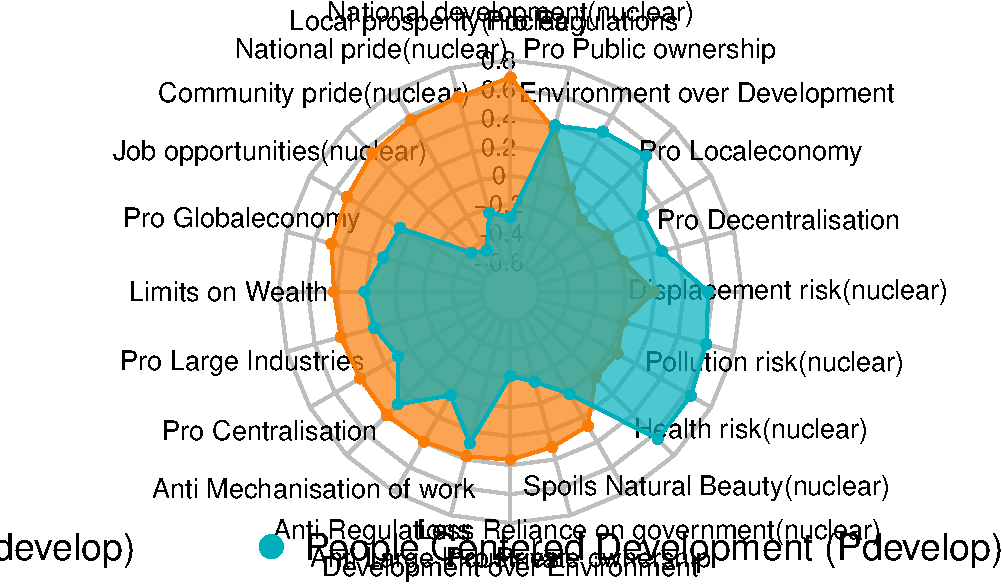
\includegraphics[width=1\linewidth,height=1\textheight]{withmice_files/figure-latex/unnamed-chunk-21-1}

\begin{landscape}
\newpage

\hypertarget{pretty-table-nuclear-efa}{%
\subsection{Pretty table: Nuclear EFA}\label{pretty-table-nuclear-efa}}

\global\setlength{\Oldarrayrulewidth}{\arrayrulewidth}

\global\setlength{\Oldtabcolsep}{\tabcolsep}

\setlength{\tabcolsep}{0pt}

\renewcommand*{\arraystretch}{1.5}



\providecommand{\ascline}[3]{\noalign{\global\arrayrulewidth #1}\arrayrulecolor[HTML]{#2}\cline{#3}}

\begin{longtable}[c]{|p{1.50in}|p{4.50in}|p{0.75in}|p{0.75in}|p{0.75in}|p{0.75in}|p{0.75in}}

\caption{Table\ 3:\ EFA\ on\ Eco-Pol\ Values\ Scale}\\

\ascline{1.5pt}{666666}{1-7}

\multicolumn{1}{>{\raggedright}m{\dimexpr 1.5in+0\tabcolsep}}{\textcolor[HTML]{000000}{\fontsize{10}{10}\selectfont{\global\setmainfont{Helvetica}{code}}}} & \multicolumn{1}{>{\raggedright}m{\dimexpr 4.5in+0\tabcolsep}}{\textcolor[HTML]{000000}{\fontsize{10}{10}\selectfont{\global\setmainfont{Helvetica}{Items}}}} & \multicolumn{1}{>{\raggedright}m{\dimexpr 0.75in+0\tabcolsep}}{\textcolor[HTML]{000000}{\fontsize{10}{10}\selectfont{\global\setmainfont{Helvetica}{Ndevelop}}}} & \multicolumn{1}{>{\raggedright}m{\dimexpr 0.75in+0\tabcolsep}}{\textcolor[HTML]{000000}{\fontsize{10}{10}\selectfont{\global\setmainfont{Helvetica}{Pdevelop}}}} & \multicolumn{1}{>{\raggedleft}m{\dimexpr 0.75in+0\tabcolsep}}{\textcolor[HTML]{000000}{\fontsize{10}{10}\selectfont{\global\setmainfont{Helvetica}{Communality}}}} & \multicolumn{1}{>{\raggedleft}m{\dimexpr 0.75in+0\tabcolsep}}{\textcolor[HTML]{000000}{\fontsize{10}{10}\selectfont{\global\setmainfont{Helvetica}{Uniqueness}}}} & \multicolumn{1}{>{\raggedleft}m{\dimexpr 0.75in+0\tabcolsep}}{\textcolor[HTML]{000000}{\fontsize{10}{10}\selectfont{\global\setmainfont{Helvetica}{Complexity}}}} \\

\ascline{1.5pt}{666666}{1-7}\endfirsthead \caption[]{Table\ 3:\ EFA\ on\ Eco-Pol\ Values\ Scale}\\

\ascline{1.5pt}{666666}{1-7}

\multicolumn{1}{>{\raggedright}m{\dimexpr 1.5in+0\tabcolsep}}{\textcolor[HTML]{000000}{\fontsize{10}{10}\selectfont{\global\setmainfont{Helvetica}{code}}}} & \multicolumn{1}{>{\raggedright}m{\dimexpr 4.5in+0\tabcolsep}}{\textcolor[HTML]{000000}{\fontsize{10}{10}\selectfont{\global\setmainfont{Helvetica}{Items}}}} & \multicolumn{1}{>{\raggedright}m{\dimexpr 0.75in+0\tabcolsep}}{\textcolor[HTML]{000000}{\fontsize{10}{10}\selectfont{\global\setmainfont{Helvetica}{Ndevelop}}}} & \multicolumn{1}{>{\raggedright}m{\dimexpr 0.75in+0\tabcolsep}}{\textcolor[HTML]{000000}{\fontsize{10}{10}\selectfont{\global\setmainfont{Helvetica}{Pdevelop}}}} & \multicolumn{1}{>{\raggedleft}m{\dimexpr 0.75in+0\tabcolsep}}{\textcolor[HTML]{000000}{\fontsize{10}{10}\selectfont{\global\setmainfont{Helvetica}{Communality}}}} & \multicolumn{1}{>{\raggedleft}m{\dimexpr 0.75in+0\tabcolsep}}{\textcolor[HTML]{000000}{\fontsize{10}{10}\selectfont{\global\setmainfont{Helvetica}{Uniqueness}}}} & \multicolumn{1}{>{\raggedleft}m{\dimexpr 0.75in+0\tabcolsep}}{\textcolor[HTML]{000000}{\fontsize{10}{10}\selectfont{\global\setmainfont{Helvetica}{Complexity}}}} \\

\ascline{1.5pt}{666666}{1-7}\endhead



\multicolumn{1}{>{\raggedright}m{\dimexpr 1.5in+0\tabcolsep}}{\textcolor[HTML]{000000}{\fontsize{10}{10}\selectfont{\global\setmainfont{Helvetica}{National\ development(nuclear)}}}} & \multicolumn{1}{>{\raggedright}m{\dimexpr 4.5in+0\tabcolsep}}{\textcolor[HTML]{000000}{\fontsize{10}{10}\selectfont{\global\setmainfont{Helvetica}{Nuclear\ energy\ pushes\ forward\ the\ country's\ development}}}} & \multicolumn{1}{>{\raggedright}m{\dimexpr 0.75in+0\tabcolsep}}{\textcolor[HTML]{000000}{\fontsize{10}{10}\selectfont{\global\setmainfont{Helvetica}{0.681}}}} & \multicolumn{1}{>{\raggedright}m{\dimexpr 0.75in+0\tabcolsep}}{\textcolor[HTML]{000000}{\fontsize{10}{10}\selectfont{\global\setmainfont{Helvetica}{}}}} & \multicolumn{1}{>{\raggedleft}m{\dimexpr 0.75in+0\tabcolsep}}{\textcolor[HTML]{000000}{\fontsize{10}{10}\selectfont{\global\setmainfont{Helvetica}{0.544}}}} & \multicolumn{1}{>{\raggedleft}m{\dimexpr 0.75in+0\tabcolsep}}{\textcolor[HTML]{000000}{\fontsize{10}{10}\selectfont{\global\setmainfont{Helvetica}{0.456}}}} & \multicolumn{1}{>{\raggedleft}m{\dimexpr 0.75in+0\tabcolsep}}{\textcolor[HTML]{000000}{\fontsize{10}{10}\selectfont{\global\setmainfont{Helvetica}{1.338}}}} \\





\multicolumn{1}{>{\raggedright}m{\dimexpr 1.5in+0\tabcolsep}}{\textcolor[HTML]{000000}{\fontsize{10}{10}\selectfont{\global\setmainfont{Helvetica}{Local\ prosperity(nuclear)}}}} & \multicolumn{1}{>{\raggedright}m{\dimexpr 4.5in+0\tabcolsep}}{\textcolor[HTML]{000000}{\fontsize{10}{10}\selectfont{\global\setmainfont{Helvetica}{Nuclear\ energy\ brings\ economic\ prosperity\ to\ the\ surrounding\ regions}}}} & \multicolumn{1}{>{\raggedright}m{\dimexpr 0.75in+0\tabcolsep}}{\textcolor[HTML]{000000}{\fontsize{10}{10}\selectfont{\global\setmainfont{Helvetica}{0.593}}}} & \multicolumn{1}{>{\raggedright}m{\dimexpr 0.75in+0\tabcolsep}}{\textcolor[HTML]{000000}{\fontsize{10}{10}\selectfont{\global\setmainfont{Helvetica}{}}}} & \multicolumn{1}{>{\raggedleft}m{\dimexpr 0.75in+0\tabcolsep}}{\textcolor[HTML]{000000}{\fontsize{10}{10}\selectfont{\global\setmainfont{Helvetica}{0.407}}}} & \multicolumn{1}{>{\raggedleft}m{\dimexpr 0.75in+0\tabcolsep}}{\textcolor[HTML]{000000}{\fontsize{10}{10}\selectfont{\global\setmainfont{Helvetica}{0.593}}}} & \multicolumn{1}{>{\raggedleft}m{\dimexpr 0.75in+0\tabcolsep}}{\textcolor[HTML]{000000}{\fontsize{10}{10}\selectfont{\global\setmainfont{Helvetica}{1.307}}}} \\





\multicolumn{1}{>{\raggedright}m{\dimexpr 1.5in+0\tabcolsep}}{\textcolor[HTML]{000000}{\fontsize{10}{10}\selectfont{\global\setmainfont{Helvetica}{National\ pride(nuclear)}}}} & \multicolumn{1}{>{\raggedright}m{\dimexpr 4.5in+0\tabcolsep}}{\textcolor[HTML]{000000}{\fontsize{10}{10}\selectfont{\global\setmainfont{Helvetica}{Nuclear\ energy\ is\ a\ mark\ of\ pride\ for\ our\ nation}}}} & \multicolumn{1}{>{\raggedright}m{\dimexpr 0.75in+0\tabcolsep}}{\textcolor[HTML]{000000}{\fontsize{10}{10}\selectfont{\global\setmainfont{Helvetica}{0.571}}}} & \multicolumn{1}{>{\raggedright}m{\dimexpr 0.75in+0\tabcolsep}}{\textcolor[HTML]{000000}{\fontsize{10}{10}\selectfont{\global\setmainfont{Helvetica}{-0.472}}}} & \multicolumn{1}{>{\raggedleft}m{\dimexpr 0.75in+0\tabcolsep}}{\textcolor[HTML]{000000}{\fontsize{10}{10}\selectfont{\global\setmainfont{Helvetica}{0.548}}}} & \multicolumn{1}{>{\raggedleft}m{\dimexpr 0.75in+0\tabcolsep}}{\textcolor[HTML]{000000}{\fontsize{10}{10}\selectfont{\global\setmainfont{Helvetica}{0.452}}}} & \multicolumn{1}{>{\raggedleft}m{\dimexpr 0.75in+0\tabcolsep}}{\textcolor[HTML]{000000}{\fontsize{10}{10}\selectfont{\global\setmainfont{Helvetica}{1.932}}}} \\





\multicolumn{1}{>{\raggedright}m{\dimexpr 1.5in+0\tabcolsep}}{\textcolor[HTML]{000000}{\fontsize{10}{10}\selectfont{\global\setmainfont{Helvetica}{Community\ pride(nuclear)}}}} & \multicolumn{1}{>{\raggedright}m{\dimexpr 4.5in+0\tabcolsep}}{\textcolor[HTML]{000000}{\fontsize{10}{10}\selectfont{\global\setmainfont{Helvetica}{I\ would\ be\ proud\ if\ my\ community\ used\ nuclear\ energy}}}} & \multicolumn{1}{>{\raggedright}m{\dimexpr 0.75in+0\tabcolsep}}{\textcolor[HTML]{000000}{\fontsize{10}{10}\selectfont{\global\setmainfont{Helvetica}{0.552}}}} & \multicolumn{1}{>{\raggedright}m{\dimexpr 0.75in+0\tabcolsep}}{\textcolor[HTML]{000000}{\fontsize{10}{10}\selectfont{\global\setmainfont{Helvetica}{-0.419}}}} & \multicolumn{1}{>{\raggedleft}m{\dimexpr 0.75in+0\tabcolsep}}{\textcolor[HTML]{000000}{\fontsize{10}{10}\selectfont{\global\setmainfont{Helvetica}{0.480}}}} & \multicolumn{1}{>{\raggedleft}m{\dimexpr 0.75in+0\tabcolsep}}{\textcolor[HTML]{000000}{\fontsize{10}{10}\selectfont{\global\setmainfont{Helvetica}{0.520}}}} & \multicolumn{1}{>{\raggedleft}m{\dimexpr 0.75in+0\tabcolsep}}{\textcolor[HTML]{000000}{\fontsize{10}{10}\selectfont{\global\setmainfont{Helvetica}{1.866}}}} \\





\multicolumn{1}{>{\raggedright}m{\dimexpr 1.5in+0\tabcolsep}}{\textcolor[HTML]{000000}{\fontsize{10}{10}\selectfont{\global\setmainfont{Helvetica}{Job\ opportunities(nuclear)}}}} & \multicolumn{1}{>{\raggedright}m{\dimexpr 4.5in+0\tabcolsep}}{\textcolor[HTML]{000000}{\fontsize{10}{10}\selectfont{\global\setmainfont{Helvetica}{Nuclear\ energy\ will\ bring\ jobs\ to\ the\ local\ community}}}} & \multicolumn{1}{>{\raggedright}m{\dimexpr 0.75in+0\tabcolsep}}{\textcolor[HTML]{000000}{\fontsize{10}{10}\selectfont{\global\setmainfont{Helvetica}{0.505}}}} & \multicolumn{1}{>{\raggedright}m{\dimexpr 0.75in+0\tabcolsep}}{\textcolor[HTML]{000000}{\fontsize{10}{10}\selectfont{\global\setmainfont{Helvetica}{}}}} & \multicolumn{1}{>{\raggedleft}m{\dimexpr 0.75in+0\tabcolsep}}{\textcolor[HTML]{000000}{\fontsize{10}{10}\selectfont{\global\setmainfont{Helvetica}{0.262}}}} & \multicolumn{1}{>{\raggedleft}m{\dimexpr 0.75in+0\tabcolsep}}{\textcolor[HTML]{000000}{\fontsize{10}{10}\selectfont{\global\setmainfont{Helvetica}{0.738}}}} & \multicolumn{1}{>{\raggedleft}m{\dimexpr 0.75in+0\tabcolsep}}{\textcolor[HTML]{000000}{\fontsize{10}{10}\selectfont{\global\setmainfont{Helvetica}{1.050}}}} \\





\multicolumn{1}{>{\raggedright}m{\dimexpr 1.5in+0\tabcolsep}}{\textcolor[HTML]{000000}{\fontsize{10}{10}\selectfont{\global\setmainfont{Helvetica}{Pro\ Globaleconomy}}}} & \multicolumn{1}{>{\raggedright}m{\dimexpr 4.5in+0\tabcolsep}}{\textcolor[HTML]{000000}{\fontsize{10}{10}\selectfont{\global\setmainfont{Helvetica}{Foreign\ companies\ have\ led\ to\ a\ range\ of\ benefits\ for\ the\ Indian\ people\ and\ society}}}} & \multicolumn{1}{>{\raggedright}m{\dimexpr 0.75in+0\tabcolsep}}{\textcolor[HTML]{000000}{\fontsize{10}{10}\selectfont{\global\setmainfont{Helvetica}{0.481}}}} & \multicolumn{1}{>{\raggedright}m{\dimexpr 0.75in+0\tabcolsep}}{\textcolor[HTML]{000000}{\fontsize{10}{10}\selectfont{\global\setmainfont{Helvetica}{}}}} & \multicolumn{1}{>{\raggedleft}m{\dimexpr 0.75in+0\tabcolsep}}{\textcolor[HTML]{000000}{\fontsize{10}{10}\selectfont{\global\setmainfont{Helvetica}{0.244}}}} & \multicolumn{1}{>{\raggedleft}m{\dimexpr 0.75in+0\tabcolsep}}{\textcolor[HTML]{000000}{\fontsize{10}{10}\selectfont{\global\setmainfont{Helvetica}{0.756}}}} & \multicolumn{1}{>{\raggedleft}m{\dimexpr 0.75in+0\tabcolsep}}{\textcolor[HTML]{000000}{\fontsize{10}{10}\selectfont{\global\setmainfont{Helvetica}{1.108}}}} \\





\multicolumn{1}{>{\raggedright}m{\dimexpr 1.5in+0\tabcolsep}}{\textcolor[HTML]{000000}{\fontsize{10}{10}\selectfont{\global\setmainfont{Helvetica}{Limits\ on\ Wealth}}}} & \multicolumn{1}{>{\raggedright}m{\dimexpr 4.5in+0\tabcolsep}}{\textcolor[HTML]{000000}{\fontsize{10}{10}\selectfont{\global\setmainfont{Helvetica}{A\ limit\ should\ be\ put\ to\ how\ much\ wealth\ a\ person\ can\ amass}}}} & \multicolumn{1}{>{\raggedright}m{\dimexpr 0.75in+0\tabcolsep}}{\textcolor[HTML]{000000}{\fontsize{10}{10}\selectfont{\global\setmainfont{Helvetica}{0.419}}}} & \multicolumn{1}{>{\raggedright}m{\dimexpr 0.75in+0\tabcolsep}}{\textcolor[HTML]{000000}{\fontsize{10}{10}\selectfont{\global\setmainfont{Helvetica}{}}}} & \multicolumn{1}{>{\raggedleft}m{\dimexpr 0.75in+0\tabcolsep}}{\textcolor[HTML]{000000}{\fontsize{10}{10}\selectfont{\global\setmainfont{Helvetica}{0.219}}}} & \multicolumn{1}{>{\raggedleft}m{\dimexpr 0.75in+0\tabcolsep}}{\textcolor[HTML]{000000}{\fontsize{10}{10}\selectfont{\global\setmainfont{Helvetica}{0.781}}}} & \multicolumn{1}{>{\raggedleft}m{\dimexpr 0.75in+0\tabcolsep}}{\textcolor[HTML]{000000}{\fontsize{10}{10}\selectfont{\global\setmainfont{Helvetica}{1.466}}}} \\





\multicolumn{1}{>{\raggedright}m{\dimexpr 1.5in+0\tabcolsep}}{\textcolor[HTML]{000000}{\fontsize{10}{10}\selectfont{\global\setmainfont{Helvetica}{Pro\ Large\ Industries}}}} & \multicolumn{1}{>{\raggedright}m{\dimexpr 4.5in+0\tabcolsep}}{\textcolor[HTML]{000000}{\fontsize{10}{10}\selectfont{\global\setmainfont{Helvetica}{Large\ scale\ industries\ are\ required\ for\ the\ development\ of\ the\ country\ that\ will\ benefit\ everyone}}}} & \multicolumn{1}{>{\raggedright}m{\dimexpr 0.75in+0\tabcolsep}}{\textcolor[HTML]{000000}{\fontsize{10}{10}\selectfont{\global\setmainfont{Helvetica}{0.415}}}} & \multicolumn{1}{>{\raggedright}m{\dimexpr 0.75in+0\tabcolsep}}{\textcolor[HTML]{000000}{\fontsize{10}{10}\selectfont{\global\setmainfont{Helvetica}{}}}} & \multicolumn{1}{>{\raggedleft}m{\dimexpr 0.75in+0\tabcolsep}}{\textcolor[HTML]{000000}{\fontsize{10}{10}\selectfont{\global\setmainfont{Helvetica}{0.202}}}} & \multicolumn{1}{>{\raggedleft}m{\dimexpr 0.75in+0\tabcolsep}}{\textcolor[HTML]{000000}{\fontsize{10}{10}\selectfont{\global\setmainfont{Helvetica}{0.798}}}} & \multicolumn{1}{>{\raggedleft}m{\dimexpr 0.75in+0\tabcolsep}}{\textcolor[HTML]{000000}{\fontsize{10}{10}\selectfont{\global\setmainfont{Helvetica}{1.338}}}} \\





\multicolumn{1}{>{\raggedright}m{\dimexpr 1.5in+0\tabcolsep}}{\textcolor[HTML]{000000}{\fontsize{10}{10}\selectfont{\global\setmainfont{Helvetica}{Anti\ Mechanisation\ of\ work}}}} & \multicolumn{1}{>{\raggedright}m{\dimexpr 4.5in+0\tabcolsep}}{\textcolor[HTML]{000000}{\fontsize{10}{10}\selectfont{\global\setmainfont{Helvetica}{Rapid\ mechanization\ of\ work\ is\ taking\ away\ jobs\ from\ workers\ in\ this\ country}}}} & \multicolumn{1}{>{\raggedright}m{\dimexpr 0.75in+0\tabcolsep}}{\textcolor[HTML]{000000}{\fontsize{10}{10}\selectfont{\global\setmainfont{Helvetica}{0.409}}}} & \multicolumn{1}{>{\raggedright}m{\dimexpr 0.75in+0\tabcolsep}}{\textcolor[HTML]{000000}{\fontsize{10}{10}\selectfont{\global\setmainfont{Helvetica}{}}}} & \multicolumn{1}{>{\raggedleft}m{\dimexpr 0.75in+0\tabcolsep}}{\textcolor[HTML]{000000}{\fontsize{10}{10}\selectfont{\global\setmainfont{Helvetica}{0.258}}}} & \multicolumn{1}{>{\raggedleft}m{\dimexpr 0.75in+0\tabcolsep}}{\textcolor[HTML]{000000}{\fontsize{10}{10}\selectfont{\global\setmainfont{Helvetica}{0.742}}}} & \multicolumn{1}{>{\raggedleft}m{\dimexpr 0.75in+0\tabcolsep}}{\textcolor[HTML]{000000}{\fontsize{10}{10}\selectfont{\global\setmainfont{Helvetica}{1.839}}}} \\





\multicolumn{1}{>{\raggedright}m{\dimexpr 1.5in+0\tabcolsep}}{\textcolor[HTML]{000000}{\fontsize{10}{10}\selectfont{\global\setmainfont{Helvetica}{Pro\ Centralisation}}}} & \multicolumn{1}{>{\raggedright}m{\dimexpr 4.5in+0\tabcolsep}}{\textcolor[HTML]{000000}{\fontsize{10}{10}\selectfont{\global\setmainfont{Helvetica}{Laws\ and\ policies\ would\ be\ implemented\ more\ smoothly\ if\ more\ power\ lay\ with\ the\ central\ government}}}} & \multicolumn{1}{>{\raggedright}m{\dimexpr 0.75in+0\tabcolsep}}{\textcolor[HTML]{000000}{\fontsize{10}{10}\selectfont{\global\setmainfont{Helvetica}{}}}} & \multicolumn{1}{>{\raggedright}m{\dimexpr 0.75in+0\tabcolsep}}{\textcolor[HTML]{000000}{\fontsize{10}{10}\selectfont{\global\setmainfont{Helvetica}{}}}} & \multicolumn{1}{>{\raggedleft}m{\dimexpr 0.75in+0\tabcolsep}}{\textcolor[HTML]{000000}{\fontsize{10}{10}\selectfont{\global\setmainfont{Helvetica}{0.169}}}} & \multicolumn{1}{>{\raggedleft}m{\dimexpr 0.75in+0\tabcolsep}}{\textcolor[HTML]{000000}{\fontsize{10}{10}\selectfont{\global\setmainfont{Helvetica}{0.831}}}} & \multicolumn{1}{>{\raggedleft}m{\dimexpr 0.75in+0\tabcolsep}}{\textcolor[HTML]{000000}{\fontsize{10}{10}\selectfont{\global\setmainfont{Helvetica}{1.114}}}} \\





\multicolumn{1}{>{\raggedright}m{\dimexpr 1.5in+0\tabcolsep}}{\textcolor[HTML]{000000}{\fontsize{10}{10}\selectfont{\global\setmainfont{Helvetica}{Anti\ Regulations}}}} & \multicolumn{1}{>{\raggedright}m{\dimexpr 4.5in+0\tabcolsep}}{\textcolor[HTML]{000000}{\fontsize{10}{10}\selectfont{\global\setmainfont{Helvetica}{There\ is\ too\ much\ red-tape\ and\ the\ government\ should\ not\ interfere\ with\ businesses\ and\ industries}}}} & \multicolumn{1}{>{\raggedright}m{\dimexpr 0.75in+0\tabcolsep}}{\textcolor[HTML]{000000}{\fontsize{10}{10}\selectfont{\global\setmainfont{Helvetica}{}}}} & \multicolumn{1}{>{\raggedright}m{\dimexpr 0.75in+0\tabcolsep}}{\textcolor[HTML]{000000}{\fontsize{10}{10}\selectfont{\global\setmainfont{Helvetica}{}}}} & \multicolumn{1}{>{\raggedleft}m{\dimexpr 0.75in+0\tabcolsep}}{\textcolor[HTML]{000000}{\fontsize{10}{10}\selectfont{\global\setmainfont{Helvetica}{0.159}}}} & \multicolumn{1}{>{\raggedleft}m{\dimexpr 0.75in+0\tabcolsep}}{\textcolor[HTML]{000000}{\fontsize{10}{10}\selectfont{\global\setmainfont{Helvetica}{0.841}}}} & \multicolumn{1}{>{\raggedleft}m{\dimexpr 0.75in+0\tabcolsep}}{\textcolor[HTML]{000000}{\fontsize{10}{10}\selectfont{\global\setmainfont{Helvetica}{1.009}}}} \\





\multicolumn{1}{>{\raggedright}m{\dimexpr 1.5in+0\tabcolsep}}{\textcolor[HTML]{000000}{\fontsize{10}{10}\selectfont{\global\setmainfont{Helvetica}{Anti\ Large\ Industries}}}} & \multicolumn{1}{>{\raggedright}m{\dimexpr 4.5in+0\tabcolsep}}{\textcolor[HTML]{000000}{\fontsize{10}{10}\selectfont{\global\setmainfont{Helvetica}{Large\ corporations\ are\ destroying\ the\ local\ industries\ in\ India\ and\ benefiting\ only\ a\ handful\ of\ people}}}} & \multicolumn{1}{>{\raggedright}m{\dimexpr 0.75in+0\tabcolsep}}{\textcolor[HTML]{000000}{\fontsize{10}{10}\selectfont{\global\setmainfont{Helvetica}{}}}} & \multicolumn{1}{>{\raggedright}m{\dimexpr 0.75in+0\tabcolsep}}{\textcolor[HTML]{000000}{\fontsize{10}{10}\selectfont{\global\setmainfont{Helvetica}{}}}} & \multicolumn{1}{>{\raggedleft}m{\dimexpr 0.75in+0\tabcolsep}}{\textcolor[HTML]{000000}{\fontsize{10}{10}\selectfont{\global\setmainfont{Helvetica}{0.224}}}} & \multicolumn{1}{>{\raggedleft}m{\dimexpr 0.75in+0\tabcolsep}}{\textcolor[HTML]{000000}{\fontsize{10}{10}\selectfont{\global\setmainfont{Helvetica}{0.776}}}} & \multicolumn{1}{>{\raggedleft}m{\dimexpr 0.75in+0\tabcolsep}}{\textcolor[HTML]{000000}{\fontsize{10}{10}\selectfont{\global\setmainfont{Helvetica}{1.859}}}} \\





\multicolumn{1}{>{\raggedright}m{\dimexpr 1.5in+0\tabcolsep}}{\textcolor[HTML]{000000}{\fontsize{10}{10}\selectfont{\global\setmainfont{Helvetica}{Development\ over\ Environment}}}} & \multicolumn{1}{>{\raggedright}m{\dimexpr 4.5in+0\tabcolsep}}{\textcolor[HTML]{000000}{\fontsize{10}{10}\selectfont{\global\setmainfont{Helvetica}{Economic\ growth\ and\ creating\ jobs\ should\ be\ prioritized\ over\ environmental\ protection}}}} & \multicolumn{1}{>{\raggedright}m{\dimexpr 0.75in+0\tabcolsep}}{\textcolor[HTML]{000000}{\fontsize{10}{10}\selectfont{\global\setmainfont{Helvetica}{}}}} & \multicolumn{1}{>{\raggedright}m{\dimexpr 0.75in+0\tabcolsep}}{\textcolor[HTML]{000000}{\fontsize{10}{10}\selectfont{\global\setmainfont{Helvetica}{}}}} & \multicolumn{1}{>{\raggedleft}m{\dimexpr 0.75in+0\tabcolsep}}{\textcolor[HTML]{000000}{\fontsize{10}{10}\selectfont{\global\setmainfont{Helvetica}{0.177}}}} & \multicolumn{1}{>{\raggedleft}m{\dimexpr 0.75in+0\tabcolsep}}{\textcolor[HTML]{000000}{\fontsize{10}{10}\selectfont{\global\setmainfont{Helvetica}{0.823}}}} & \multicolumn{1}{>{\raggedleft}m{\dimexpr 0.75in+0\tabcolsep}}{\textcolor[HTML]{000000}{\fontsize{10}{10}\selectfont{\global\setmainfont{Helvetica}{1.639}}}} \\





\multicolumn{1}{>{\raggedright}m{\dimexpr 1.5in+0\tabcolsep}}{\textcolor[HTML]{000000}{\fontsize{10}{10}\selectfont{\global\setmainfont{Helvetica}{Pro\ Private\ ownership}}}} & \multicolumn{1}{>{\raggedright}m{\dimexpr 4.5in+0\tabcolsep}}{\textcolor[HTML]{000000}{\fontsize{10}{10}\selectfont{\global\setmainfont{Helvetica}{All\ businesses\ and\ industries\ should\ be\ owned\ privately}}}} & \multicolumn{1}{>{\raggedright}m{\dimexpr 0.75in+0\tabcolsep}}{\textcolor[HTML]{000000}{\fontsize{10}{10}\selectfont{\global\setmainfont{Helvetica}{}}}} & \multicolumn{1}{>{\raggedright}m{\dimexpr 0.75in+0\tabcolsep}}{\textcolor[HTML]{000000}{\fontsize{10}{10}\selectfont{\global\setmainfont{Helvetica}{}}}} & \multicolumn{1}{>{\raggedleft}m{\dimexpr 0.75in+0\tabcolsep}}{\textcolor[HTML]{000000}{\fontsize{10}{10}\selectfont{\global\setmainfont{Helvetica}{0.122}}}} & \multicolumn{1}{>{\raggedleft}m{\dimexpr 0.75in+0\tabcolsep}}{\textcolor[HTML]{000000}{\fontsize{10}{10}\selectfont{\global\setmainfont{Helvetica}{0.878}}}} & \multicolumn{1}{>{\raggedleft}m{\dimexpr 0.75in+0\tabcolsep}}{\textcolor[HTML]{000000}{\fontsize{10}{10}\selectfont{\global\setmainfont{Helvetica}{1.467}}}} \\





\multicolumn{1}{>{\raggedright}m{\dimexpr 1.5in+0\tabcolsep}}{\textcolor[HTML]{000000}{\fontsize{10}{10}\selectfont{\global\setmainfont{Helvetica}{Less\ Reliance\ on\ government(nuclear)}}}} & \multicolumn{1}{>{\raggedright}m{\dimexpr 4.5in+0\tabcolsep}}{\textcolor[HTML]{000000}{\fontsize{10}{10}\selectfont{\global\setmainfont{Helvetica}{I\ don't\ like\ the\ idea\ that\ I\ have\ to\ rely\ on\ the\ government\ for\ electricity\ from\ nuclear\ energy}}}} & \multicolumn{1}{>{\raggedright}m{\dimexpr 0.75in+0\tabcolsep}}{\textcolor[HTML]{000000}{\fontsize{10}{10}\selectfont{\global\setmainfont{Helvetica}{}}}} & \multicolumn{1}{>{\raggedright}m{\dimexpr 0.75in+0\tabcolsep}}{\textcolor[HTML]{000000}{\fontsize{10}{10}\selectfont{\global\setmainfont{Helvetica}{}}}} & \multicolumn{1}{>{\raggedleft}m{\dimexpr 0.75in+0\tabcolsep}}{\textcolor[HTML]{000000}{\fontsize{10}{10}\selectfont{\global\setmainfont{Helvetica}{0.074}}}} & \multicolumn{1}{>{\raggedleft}m{\dimexpr 0.75in+0\tabcolsep}}{\textcolor[HTML]{000000}{\fontsize{10}{10}\selectfont{\global\setmainfont{Helvetica}{0.926}}}} & \multicolumn{1}{>{\raggedleft}m{\dimexpr 0.75in+0\tabcolsep}}{\textcolor[HTML]{000000}{\fontsize{10}{10}\selectfont{\global\setmainfont{Helvetica}{1.008}}}} \\





\multicolumn{1}{>{\raggedright}m{\dimexpr 1.5in+0\tabcolsep}}{\textcolor[HTML]{000000}{\fontsize{10}{10}\selectfont{\global\setmainfont{Helvetica}{Health\ risk(nuclear)}}}} & \multicolumn{1}{>{\raggedright}m{\dimexpr 4.5in+0\tabcolsep}}{\textcolor[HTML]{000000}{\fontsize{10}{10}\selectfont{\global\setmainfont{Helvetica}{Nuclear\ energy\ poses\ a\ great\ risk\ to\ the\ health\ of\ people\ living\ around\ it}}}} & \multicolumn{1}{>{\raggedright}m{\dimexpr 0.75in+0\tabcolsep}}{\textcolor[HTML]{000000}{\fontsize{10}{10}\selectfont{\global\setmainfont{Helvetica}{}}}} & \multicolumn{1}{>{\raggedright}m{\dimexpr 0.75in+0\tabcolsep}}{\textcolor[HTML]{000000}{\fontsize{10}{10}\selectfont{\global\setmainfont{Helvetica}{0.639}}}} & \multicolumn{1}{>{\raggedleft}m{\dimexpr 0.75in+0\tabcolsep}}{\textcolor[HTML]{000000}{\fontsize{10}{10}\selectfont{\global\setmainfont{Helvetica}{0.412}}}} & \multicolumn{1}{>{\raggedleft}m{\dimexpr 0.75in+0\tabcolsep}}{\textcolor[HTML]{000000}{\fontsize{10}{10}\selectfont{\global\setmainfont{Helvetica}{0.588}}}} & \multicolumn{1}{>{\raggedleft}m{\dimexpr 0.75in+0\tabcolsep}}{\textcolor[HTML]{000000}{\fontsize{10}{10}\selectfont{\global\setmainfont{Helvetica}{1.015}}}} \\





\multicolumn{1}{>{\raggedright}m{\dimexpr 1.5in+0\tabcolsep}}{\textcolor[HTML]{000000}{\fontsize{10}{10}\selectfont{\global\setmainfont{Helvetica}{Spoils\ Natural\ Beauty(nuclear)}}}} & \multicolumn{1}{>{\raggedright}m{\dimexpr 4.5in+0\tabcolsep}}{\textcolor[HTML]{000000}{\fontsize{10}{10}\selectfont{\global\setmainfont{Helvetica}{Nuclear\ energy\ spoils\ the\ natural\ beauty\ of\ the\ landscape}}}} & \multicolumn{1}{>{\raggedright}m{\dimexpr 0.75in+0\tabcolsep}}{\textcolor[HTML]{000000}{\fontsize{10}{10}\selectfont{\global\setmainfont{Helvetica}{}}}} & \multicolumn{1}{>{\raggedright}m{\dimexpr 0.75in+0\tabcolsep}}{\textcolor[HTML]{000000}{\fontsize{10}{10}\selectfont{\global\setmainfont{Helvetica}{0.639}}}} & \multicolumn{1}{>{\raggedleft}m{\dimexpr 0.75in+0\tabcolsep}}{\textcolor[HTML]{000000}{\fontsize{10}{10}\selectfont{\global\setmainfont{Helvetica}{0.410}}}} & \multicolumn{1}{>{\raggedleft}m{\dimexpr 0.75in+0\tabcolsep}}{\textcolor[HTML]{000000}{\fontsize{10}{10}\selectfont{\global\setmainfont{Helvetica}{0.590}}}} & \multicolumn{1}{>{\raggedleft}m{\dimexpr 0.75in+0\tabcolsep}}{\textcolor[HTML]{000000}{\fontsize{10}{10}\selectfont{\global\setmainfont{Helvetica}{1.005}}}} \\





\multicolumn{1}{>{\raggedright}m{\dimexpr 1.5in+0\tabcolsep}}{\textcolor[HTML]{000000}{\fontsize{10}{10}\selectfont{\global\setmainfont{Helvetica}{Pollution\ risk(nuclear)}}}} & \multicolumn{1}{>{\raggedright}m{\dimexpr 4.5in+0\tabcolsep}}{\textcolor[HTML]{000000}{\fontsize{10}{10}\selectfont{\global\setmainfont{Helvetica}{Nuclear\ energy\ increases\ pollution\ of\ air/water/land}}}} & \multicolumn{1}{>{\raggedright}m{\dimexpr 0.75in+0\tabcolsep}}{\textcolor[HTML]{000000}{\fontsize{10}{10}\selectfont{\global\setmainfont{Helvetica}{}}}} & \multicolumn{1}{>{\raggedright}m{\dimexpr 0.75in+0\tabcolsep}}{\textcolor[HTML]{000000}{\fontsize{10}{10}\selectfont{\global\setmainfont{Helvetica}{0.602}}}} & \multicolumn{1}{>{\raggedleft}m{\dimexpr 0.75in+0\tabcolsep}}{\textcolor[HTML]{000000}{\fontsize{10}{10}\selectfont{\global\setmainfont{Helvetica}{0.363}}}} & \multicolumn{1}{>{\raggedleft}m{\dimexpr 0.75in+0\tabcolsep}}{\textcolor[HTML]{000000}{\fontsize{10}{10}\selectfont{\global\setmainfont{Helvetica}{0.637}}}} & \multicolumn{1}{>{\raggedleft}m{\dimexpr 0.75in+0\tabcolsep}}{\textcolor[HTML]{000000}{\fontsize{10}{10}\selectfont{\global\setmainfont{Helvetica}{1.000}}}} \\





\multicolumn{1}{>{\raggedright}m{\dimexpr 1.5in+0\tabcolsep}}{\textcolor[HTML]{000000}{\fontsize{10}{10}\selectfont{\global\setmainfont{Helvetica}{Displacement\ risk(nuclear)}}}} & \multicolumn{1}{>{\raggedright}m{\dimexpr 4.5in+0\tabcolsep}}{\textcolor[HTML]{000000}{\fontsize{10}{10}\selectfont{\global\setmainfont{Helvetica}{Nuclear\ energy\ is\ leading\ to\ displacement\ of\ people\ from\ their\ land}}}} & \multicolumn{1}{>{\raggedright}m{\dimexpr 0.75in+0\tabcolsep}}{\textcolor[HTML]{000000}{\fontsize{10}{10}\selectfont{\global\setmainfont{Helvetica}{}}}} & \multicolumn{1}{>{\raggedright}m{\dimexpr 0.75in+0\tabcolsep}}{\textcolor[HTML]{000000}{\fontsize{10}{10}\selectfont{\global\setmainfont{Helvetica}{0.567}}}} & \multicolumn{1}{>{\raggedleft}m{\dimexpr 0.75in+0\tabcolsep}}{\textcolor[HTML]{000000}{\fontsize{10}{10}\selectfont{\global\setmainfont{Helvetica}{0.359}}}} & \multicolumn{1}{>{\raggedleft}m{\dimexpr 0.75in+0\tabcolsep}}{\textcolor[HTML]{000000}{\fontsize{10}{10}\selectfont{\global\setmainfont{Helvetica}{0.641}}}} & \multicolumn{1}{>{\raggedleft}m{\dimexpr 0.75in+0\tabcolsep}}{\textcolor[HTML]{000000}{\fontsize{10}{10}\selectfont{\global\setmainfont{Helvetica}{1.232}}}} \\





\multicolumn{1}{>{\raggedright}m{\dimexpr 1.5in+0\tabcolsep}}{\textcolor[HTML]{000000}{\fontsize{10}{10}\selectfont{\global\setmainfont{Helvetica}{Environment\ over\ Development}}}} & \multicolumn{1}{>{\raggedright}m{\dimexpr 4.5in+0\tabcolsep}}{\textcolor[HTML]{000000}{\fontsize{10}{10}\selectfont{\global\setmainfont{Helvetica}{Polluting\ industries\ that\ spoil\ the\ environment\ should\ be\ shut\ down\ even\ if\ it\ costs\ people\ their\ jobs}}}} & \multicolumn{1}{>{\raggedright}m{\dimexpr 0.75in+0\tabcolsep}}{\textcolor[HTML]{000000}{\fontsize{10}{10}\selectfont{\global\setmainfont{Helvetica}{}}}} & \multicolumn{1}{>{\raggedright}m{\dimexpr 0.75in+0\tabcolsep}}{\textcolor[HTML]{000000}{\fontsize{10}{10}\selectfont{\global\setmainfont{Helvetica}{0.527}}}} & \multicolumn{1}{>{\raggedleft}m{\dimexpr 0.75in+0\tabcolsep}}{\textcolor[HTML]{000000}{\fontsize{10}{10}\selectfont{\global\setmainfont{Helvetica}{0.288}}}} & \multicolumn{1}{>{\raggedleft}m{\dimexpr 0.75in+0\tabcolsep}}{\textcolor[HTML]{000000}{\fontsize{10}{10}\selectfont{\global\setmainfont{Helvetica}{0.712}}}} & \multicolumn{1}{>{\raggedleft}m{\dimexpr 0.75in+0\tabcolsep}}{\textcolor[HTML]{000000}{\fontsize{10}{10}\selectfont{\global\setmainfont{Helvetica}{1.075}}}} \\





\multicolumn{1}{>{\raggedright}m{\dimexpr 1.5in+0\tabcolsep}}{\textcolor[HTML]{000000}{\fontsize{10}{10}\selectfont{\global\setmainfont{Helvetica}{Pro\ Public\ ownership}}}} & \multicolumn{1}{>{\raggedright}m{\dimexpr 4.5in+0\tabcolsep}}{\textcolor[HTML]{000000}{\fontsize{10}{10}\selectfont{\global\setmainfont{Helvetica}{The\ government\ should\ own\ most\ large\ businesses\ and\ industries}}}} & \multicolumn{1}{>{\raggedright}m{\dimexpr 0.75in+0\tabcolsep}}{\textcolor[HTML]{000000}{\fontsize{10}{10}\selectfont{\global\setmainfont{Helvetica}{}}}} & \multicolumn{1}{>{\raggedright}m{\dimexpr 0.75in+0\tabcolsep}}{\textcolor[HTML]{000000}{\fontsize{10}{10}\selectfont{\global\setmainfont{Helvetica}{0.477}}}} & \multicolumn{1}{>{\raggedleft}m{\dimexpr 0.75in+0\tabcolsep}}{\textcolor[HTML]{000000}{\fontsize{10}{10}\selectfont{\global\setmainfont{Helvetica}{0.229}}}} & \multicolumn{1}{>{\raggedleft}m{\dimexpr 0.75in+0\tabcolsep}}{\textcolor[HTML]{000000}{\fontsize{10}{10}\selectfont{\global\setmainfont{Helvetica}{0.771}}}} & \multicolumn{1}{>{\raggedleft}m{\dimexpr 0.75in+0\tabcolsep}}{\textcolor[HTML]{000000}{\fontsize{10}{10}\selectfont{\global\setmainfont{Helvetica}{1.005}}}} \\





\multicolumn{1}{>{\raggedright}m{\dimexpr 1.5in+0\tabcolsep}}{\textcolor[HTML]{000000}{\fontsize{10}{10}\selectfont{\global\setmainfont{Helvetica}{Pro\ Regulations}}}} & \multicolumn{1}{>{\raggedright}m{\dimexpr 4.5in+0\tabcolsep}}{\textcolor[HTML]{000000}{\fontsize{10}{10}\selectfont{\global\setmainfont{Helvetica}{Regardless\ of\ ownership,\ the\ government\ should\ pass\ strong\ regulations\ and\ implement\ them}}}} & \multicolumn{1}{>{\raggedright}m{\dimexpr 0.75in+0\tabcolsep}}{\textcolor[HTML]{000000}{\fontsize{10}{10}\selectfont{\global\setmainfont{Helvetica}{}}}} & \multicolumn{1}{>{\raggedright}m{\dimexpr 0.75in+0\tabcolsep}}{\textcolor[HTML]{000000}{\fontsize{10}{10}\selectfont{\global\setmainfont{Helvetica}{}}}} & \multicolumn{1}{>{\raggedleft}m{\dimexpr 0.75in+0\tabcolsep}}{\textcolor[HTML]{000000}{\fontsize{10}{10}\selectfont{\global\setmainfont{Helvetica}{0.284}}}} & \multicolumn{1}{>{\raggedleft}m{\dimexpr 0.75in+0\tabcolsep}}{\textcolor[HTML]{000000}{\fontsize{10}{10}\selectfont{\global\setmainfont{Helvetica}{0.716}}}} & \multicolumn{1}{>{\raggedleft}m{\dimexpr 0.75in+0\tabcolsep}}{\textcolor[HTML]{000000}{\fontsize{10}{10}\selectfont{\global\setmainfont{Helvetica}{1.990}}}} \\





\multicolumn{1}{>{\raggedright}m{\dimexpr 1.5in+0\tabcolsep}}{\textcolor[HTML]{000000}{\fontsize{10}{10}\selectfont{\global\setmainfont{Helvetica}{Pro\ Decentralisation}}}} & \multicolumn{1}{>{\raggedright}m{\dimexpr 4.5in+0\tabcolsep}}{\textcolor[HTML]{000000}{\fontsize{10}{10}\selectfont{\global\setmainfont{Helvetica}{Local\ politicians\ shouldn't\ have\ to\ ask\ permission\ from\ the\ central\ government\ to\ implement\ policies}}}} & \multicolumn{1}{>{\raggedright}m{\dimexpr 0.75in+0\tabcolsep}}{\textcolor[HTML]{000000}{\fontsize{10}{10}\selectfont{\global\setmainfont{Helvetica}{}}}} & \multicolumn{1}{>{\raggedright}m{\dimexpr 0.75in+0\tabcolsep}}{\textcolor[HTML]{000000}{\fontsize{10}{10}\selectfont{\global\setmainfont{Helvetica}{}}}} & \multicolumn{1}{>{\raggedleft}m{\dimexpr 0.75in+0\tabcolsep}}{\textcolor[HTML]{000000}{\fontsize{10}{10}\selectfont{\global\setmainfont{Helvetica}{0.080}}}} & \multicolumn{1}{>{\raggedleft}m{\dimexpr 0.75in+0\tabcolsep}}{\textcolor[HTML]{000000}{\fontsize{10}{10}\selectfont{\global\setmainfont{Helvetica}{0.920}}}} & \multicolumn{1}{>{\raggedleft}m{\dimexpr 0.75in+0\tabcolsep}}{\textcolor[HTML]{000000}{\fontsize{10}{10}\selectfont{\global\setmainfont{Helvetica}{1.001}}}} \\





\multicolumn{1}{>{\raggedright}m{\dimexpr 1.5in+0\tabcolsep}}{\textcolor[HTML]{000000}{\fontsize{10}{10}\selectfont{\global\setmainfont{Helvetica}{Pro\ Localeconomy}}}} & \multicolumn{1}{>{\raggedright}m{\dimexpr 4.5in+0\tabcolsep}}{\textcolor[HTML]{000000}{\fontsize{10}{10}\selectfont{\global\setmainfont{Helvetica}{India\ would\ be\ better\ off\ if\ foreign\ companies\ didn't\ come\ to\ here}}}} & \multicolumn{1}{>{\raggedright}m{\dimexpr 0.75in+0\tabcolsep}}{\textcolor[HTML]{000000}{\fontsize{10}{10}\selectfont{\global\setmainfont{Helvetica}{}}}} & \multicolumn{1}{>{\raggedright}m{\dimexpr 0.75in+0\tabcolsep}}{\textcolor[HTML]{000000}{\fontsize{10}{10}\selectfont{\global\setmainfont{Helvetica}{}}}} & \multicolumn{1}{>{\raggedleft}m{\dimexpr 0.75in+0\tabcolsep}}{\textcolor[HTML]{000000}{\fontsize{10}{10}\selectfont{\global\setmainfont{Helvetica}{0.066}}}} & \multicolumn{1}{>{\raggedleft}m{\dimexpr 0.75in+0\tabcolsep}}{\textcolor[HTML]{000000}{\fontsize{10}{10}\selectfont{\global\setmainfont{Helvetica}{0.934}}}} & \multicolumn{1}{>{\raggedleft}m{\dimexpr 0.75in+0\tabcolsep}}{\textcolor[HTML]{000000}{\fontsize{10}{10}\selectfont{\global\setmainfont{Helvetica}{1.019}}}} \\

\ascline{1.5pt}{666666}{1-7}



\end{longtable}



\arrayrulecolor[HTML]{000000}

\global\setlength{\arrayrulewidth}{\Oldarrayrulewidth}

\global\setlength{\tabcolsep}{\Oldtabcolsep}

\renewcommand*{\arraystretch}{1}

\end{landscape}

\global\setlength{\Oldarrayrulewidth}{\arrayrulewidth}

\global\setlength{\Oldtabcolsep}{\tabcolsep}

\setlength{\tabcolsep}{0pt}

\renewcommand*{\arraystretch}{1.5}



\providecommand{\ascline}[3]{\noalign{\global\arrayrulewidth #1}\arrayrulecolor[HTML]{#2}\cline{#3}}

\begin{longtable}[c]{|p{0.75in}|p{0.75in}|p{0.75in}}

\caption{Table\ 4:\ Eigenvalues\ and\ Variance\ Explained\ Eco-Pol\ Scale}\\

\ascline{1.5pt}{666666}{1-3}

\multicolumn{1}{>{\raggedright}m{\dimexpr 0.75in+0\tabcolsep}}{\textcolor[HTML]{000000}{\fontsize{10}{10}\selectfont{\global\setmainfont{Helvetica}{Property}}}} & \multicolumn{1}{>{\raggedleft}m{\dimexpr 0.75in+0\tabcolsep}}{\textcolor[HTML]{000000}{\fontsize{10}{10}\selectfont{\global\setmainfont{Helvetica}{Ndevelop}}}} & \multicolumn{1}{>{\raggedleft}m{\dimexpr 0.75in+0\tabcolsep}}{\textcolor[HTML]{000000}{\fontsize{10}{10}\selectfont{\global\setmainfont{Helvetica}{Pdevelop}}}} \\

\ascline{1.5pt}{666666}{1-3}\endfirsthead \caption[]{Table\ 4:\ Eigenvalues\ and\ Variance\ Explained\ Eco-Pol\ Scale}\\

\ascline{1.5pt}{666666}{1-3}

\multicolumn{1}{>{\raggedright}m{\dimexpr 0.75in+0\tabcolsep}}{\textcolor[HTML]{000000}{\fontsize{10}{10}\selectfont{\global\setmainfont{Helvetica}{Property}}}} & \multicolumn{1}{>{\raggedleft}m{\dimexpr 0.75in+0\tabcolsep}}{\textcolor[HTML]{000000}{\fontsize{10}{10}\selectfont{\global\setmainfont{Helvetica}{Ndevelop}}}} & \multicolumn{1}{>{\raggedleft}m{\dimexpr 0.75in+0\tabcolsep}}{\textcolor[HTML]{000000}{\fontsize{10}{10}\selectfont{\global\setmainfont{Helvetica}{Pdevelop}}}} \\

\ascline{1.5pt}{666666}{1-3}\endhead



\multicolumn{1}{>{\raggedright}m{\dimexpr 0.75in+0\tabcolsep}}{\textcolor[HTML]{000000}{\fontsize{10}{10}\selectfont{\global\setmainfont{Helvetica}{SS\ loadings}}}} & \multicolumn{1}{>{\raggedleft}m{\dimexpr 0.75in+0\tabcolsep}}{\textcolor[HTML]{000000}{\fontsize{10}{10}\selectfont{\global\setmainfont{Helvetica}{3.393}}}} & \multicolumn{1}{>{\raggedleft}m{\dimexpr 0.75in+0\tabcolsep}}{\textcolor[HTML]{000000}{\fontsize{10}{10}\selectfont{\global\setmainfont{Helvetica}{3.184}}}} \\





\multicolumn{1}{>{\raggedright}m{\dimexpr 0.75in+0\tabcolsep}}{\textcolor[HTML]{000000}{\fontsize{10}{10}\selectfont{\global\setmainfont{Helvetica}{Proportion\ Var}}}} & \multicolumn{1}{>{\raggedleft}m{\dimexpr 0.75in+0\tabcolsep}}{\textcolor[HTML]{000000}{\fontsize{10}{10}\selectfont{\global\setmainfont{Helvetica}{0.141}}}} & \multicolumn{1}{>{\raggedleft}m{\dimexpr 0.75in+0\tabcolsep}}{\textcolor[HTML]{000000}{\fontsize{10}{10}\selectfont{\global\setmainfont{Helvetica}{0.133}}}} \\





\multicolumn{1}{>{\raggedright}m{\dimexpr 0.75in+0\tabcolsep}}{\textcolor[HTML]{000000}{\fontsize{10}{10}\selectfont{\global\setmainfont{Helvetica}{Cumulative\ Var}}}} & \multicolumn{1}{>{\raggedleft}m{\dimexpr 0.75in+0\tabcolsep}}{\textcolor[HTML]{000000}{\fontsize{10}{10}\selectfont{\global\setmainfont{Helvetica}{0.141}}}} & \multicolumn{1}{>{\raggedleft}m{\dimexpr 0.75in+0\tabcolsep}}{\textcolor[HTML]{000000}{\fontsize{10}{10}\selectfont{\global\setmainfont{Helvetica}{0.274}}}} \\





\multicolumn{1}{>{\raggedright}m{\dimexpr 0.75in+0\tabcolsep}}{\textcolor[HTML]{000000}{\fontsize{10}{10}\selectfont{\global\setmainfont{Helvetica}{Proportion\ Explained}}}} & \multicolumn{1}{>{\raggedleft}m{\dimexpr 0.75in+0\tabcolsep}}{\textcolor[HTML]{000000}{\fontsize{10}{10}\selectfont{\global\setmainfont{Helvetica}{0.516}}}} & \multicolumn{1}{>{\raggedleft}m{\dimexpr 0.75in+0\tabcolsep}}{\textcolor[HTML]{000000}{\fontsize{10}{10}\selectfont{\global\setmainfont{Helvetica}{0.484}}}} \\





\multicolumn{1}{>{\raggedright}m{\dimexpr 0.75in+0\tabcolsep}}{\textcolor[HTML]{000000}{\fontsize{10}{10}\selectfont{\global\setmainfont{Helvetica}{Cumulative\ Proportion}}}} & \multicolumn{1}{>{\raggedleft}m{\dimexpr 0.75in+0\tabcolsep}}{\textcolor[HTML]{000000}{\fontsize{10}{10}\selectfont{\global\setmainfont{Helvetica}{0.516}}}} & \multicolumn{1}{>{\raggedleft}m{\dimexpr 0.75in+0\tabcolsep}}{\textcolor[HTML]{000000}{\fontsize{10}{10}\selectfont{\global\setmainfont{Helvetica}{1.000}}}} \\

\ascline{1.5pt}{666666}{1-3}



\end{longtable}



\arrayrulecolor[HTML]{000000}

\global\setlength{\arrayrulewidth}{\Oldarrayrulewidth}

\global\setlength{\tabcolsep}{\Oldtabcolsep}

\renewcommand*{\arraystretch}{1}

\hypertarget{state-ns-before-mifa}{%
\section{State Ns before MIFA}\label{state-ns-before-mifa}}

\hypertarget{state-ns-after-mifa}{%
\section{State Ns after MIFA}\label{state-ns-after-mifa}}

\hypertarget{nuclear-ecopol-mean-across-imputations}{%
\subsection{Nuclear: Ecopol (Mean across
imputations)}\label{nuclear-ecopol-mean-across-imputations}}

\hypertarget{binding-datasets}{%
\subsection{Binding datasets}\label{binding-datasets}}

\hypertarget{lms-final-imputed-datasets}{%
\section{LMs : final imputed
datasets}\label{lms-final-imputed-datasets}}

\hypertarget{correlation-table}{%
\section{correlation table}\label{correlation-table}}

\hypertarget{interaction-vars-tablle}{%
\section{interaction vars tablle}\label{interaction-vars-tablle}}

\newpage
\begin{landscape}

\hypertarget{stargazer-all-lms}{%
\section{Stargazer : all LMs}\label{stargazer-all-lms}}

\begingroup\setlength{\tabcolsep}{1pt}\renewcommand{\arraystretch}{0.7}

\% Table created by stargazer v.5.2.3 by Marek Hlavac, Social Policy
Institute. E-mail: marek.hlavac at gmail.com \% Date and time: Tue, Mar
26, 2024 - 21:09:15

\begin{table}[!htbp] \centering 
  \caption{Table 6: 5 linear models: Perceived Risk of Nuclear Energy} 
  \label{} 
\begin{tabular}{@{\extracolsep{5pt}}lccccc} 
\\[-1.8ex]\hline 
\hline \\[-1.8ex] 
 & \multicolumn{5}{c}{\textit{Dependent variable:}} \\ 
\cline{2-6} 
\\[-1.8ex] & \multicolumn{5}{c}{Risky\_Nuclear} \\ 
\\[-1.8ex] & (1) & (2) & (3) & (4) & (5)\\ 
\hline \\[-1.8ex] 
 Uppercaste & 0.029 & $-$0.194$^{**}$ & $-$0.185$^{**}$ & $-$0.178$^{**}$ & $-$0.160$^{*}$ \\ 
  & (0.092) & (0.086) & (0.086) & (0.086) & (0.086) \\ 
  & & & & & \\ 
 Male & 0.148 & 0.116 & 0.116 & 0.113 & 0.119 \\ 
  & (0.093) & (0.091) & (0.090) & (0.090) & (0.088) \\ 
  & & & & & \\ 
 Hindu & $-$0.248$^{**}$ & $-$0.081 & $-$0.096 & $-$0.082 & $-$0.067 \\ 
  & (0.105) & (0.098) & (0.098) & (0.097) & (0.096) \\ 
  & & & & & \\ 
 urban\_ruralUrban & $-$0.104 & 0.108 & 0.094 & 0.098 & 0.086 \\ 
  & (0.090) & (0.092) & (0.092) & (0.092) & (0.090) \\ 
  & & & & & \\ 
 Age & $-$0.098$^{**}$ & $-$0.150$^{***}$ & $-$0.151$^{***}$ & $-$0.149$^{***}$ & $-$0.126$^{***}$ \\ 
  & (0.038) & (0.036) & (0.036) & (0.036) & (0.036) \\ 
  & & & & & \\ 
 StateWest Bengal &  & 1.360$^{***}$ & 1.280$^{***}$ & 1.228$^{***}$ & 1.074$^{***}$ \\ 
  &  & (0.120) & (0.126) & (0.126) & (0.138) \\ 
  & & & & & \\ 
 StateRajasthan &  & 0.159 & 0.116 & 0.065 & $-$0.150 \\ 
  &  & (0.131) & (0.134) & (0.134) & (0.141) \\ 
  & & & & & \\ 
 StateTamil Nadu &  & $-$0.025 & $-$0.105 & $-$0.059 & $-$0.183 \\ 
  &  & (0.120) & (0.127) & (0.128) & (0.142) \\ 
  & & & & & \\ 
 StateUttar Pradesh &  & $-$0.066 & $-$0.097 & $-$0.104 & $-$0.280$^{*}$ \\ 
  &  & (0.159) & (0.161) & (0.162) & (0.168) \\ 
  & & & & & \\ 
 Communitarian &  &  & $-$0.030 & $-$0.036 & $-$0.057 \\ 
  &  &  & (0.041) & (0.041) & (0.081) \\ 
  & & & & & \\ 
 Egalitarian &  &  & 0.118$^{***}$ & 0.091$^{**}$ & 0.287$^{***}$ \\ 
  &  &  & (0.040) & (0.041) & (0.059) \\ 
  & & & & & \\ 
 Pdevelop &  &  &  & 0.122$^{***}$ & 0.119$^{**}$ \\ 
  &  &  &  & (0.038) & (0.060) \\ 
  & & & & & \\ 
 Ndevelop &  &  &  & 0.027 & 0.106$^{*}$ \\ 
  &  &  &  & (0.038) & (0.062) \\ 
  & & & & & \\ 
 StateWest Bengal:Communitarian &  &  &  &  & 0.030 \\ 
  &  &  &  &  & (0.126) \\ 
  & & & & & \\ 
 StateRajasthan:Communitarian &  &  &  &  & $-$0.056 \\ 
  &  &  &  &  & (0.134) \\ 
  & & & & & \\ 
 StateTamil Nadu:Communitarian &  &  &  &  & 0.026 \\ 
  &  &  &  &  & (0.113) \\ 
  & & & & & \\ 
 StateUttar Pradesh:Communitarian &  &  &  &  & 0.172 \\ 
  &  &  &  &  & (0.131) \\ 
  & & & & & \\ 
 StateWest Bengal:Egalitarian &  &  &  &  & $-$0.032 \\ 
  &  &  &  &  & (0.147) \\ 
  & & & & & \\ 
 StateRajasthan:Egalitarian &  &  &  &  & $-$0.577$^{***}$ \\ 
  &  &  &  &  & (0.137) \\ 
  & & & & & \\ 
 StateTamil Nadu:Egalitarian &  &  &  &  & $-$0.437$^{***}$ \\ 
  &  &  &  &  & (0.109) \\ 
  & & & & & \\ 
 StateUttar Pradesh:Egalitarian &  &  &  &  & $-$0.250$^{*}$ \\ 
  &  &  &  &  & (0.138) \\ 
  & & & & & \\ 
 StateWest Bengal:Pdevelop &  &  &  &  & $-$0.078 \\ 
  &  &  &  &  & (0.106) \\ 
  & & & & & \\ 
 StateRajasthan:Pdevelop &  &  &  &  & 0.250$^{**}$ \\ 
  &  &  &  &  & (0.115) \\ 
  & & & & & \\ 
 StateTamil Nadu:Pdevelop &  &  &  &  & $-$0.067 \\ 
  &  &  &  &  & (0.117) \\ 
  & & & & & \\ 
 StateUttar Pradesh:Pdevelop &  &  &  &  & $-$0.180 \\ 
  &  &  &  &  & (0.122) \\ 
  & & & & & \\ 
 StateWest Bengal:Ndevelop &  &  &  &  & $-$0.051 \\ 
  &  &  &  &  & (0.113) \\ 
  & & & & & \\ 
 StateRajasthan:Ndevelop &  &  &  &  & 0.060 \\ 
  &  &  &  &  & (0.111) \\ 
  & & & & & \\ 
 StateTamil Nadu:Ndevelop &  &  &  &  & $-$0.374$^{***}$ \\ 
  &  &  &  &  & (0.113) \\ 
  & & & & & \\ 
 StateUttar Pradesh:Ndevelop &  &  &  &  & $-$0.131 \\ 
  &  &  &  &  & (0.110) \\ 
  & & & & & \\ 
 Constant & 3.737$^{***}$ & 3.455$^{***}$ & 3.517$^{***}$ & 3.510$^{***}$ & 3.559$^{***}$ \\ 
  & (0.148) & (0.140) & (0.144) & (0.143) & (0.150) \\ 
  & & & & & \\ 
\hline \\[-1.8ex] 
Observations & 839 & 839 & 839 & 839 & 839 \\ 
R$^{2}$ & 0.019 & 0.193 & 0.203 & 0.213 & 0.272 \\ 
Adjusted R$^{2}$ & 0.013 & 0.184 & 0.192 & 0.200 & 0.246 \\ 
Residual Std. Error & 1.210 (df = 833) & 1.100 (df = 829) & 1.095 (df = 827) & 1.089 (df = 825) & 1.058 (df = 809) \\ 
F Statistic & 3.175$^{***}$ (df = 5; 833) & 22.052$^{***}$ (df = 9; 829) & 19.106$^{***}$ (df = 11; 827) & 17.150$^{***}$ (df = 13; 825) & 10.423$^{***}$ (df = 29; 809) \\ 
\hline 
\hline \\[-1.8ex] 
\textit{Note:}  & \multicolumn{5}{r}{$^{*}$p$<$0.1; $^{**}$p$<$0.05; $^{***}$p$<$0.01} \\ 
\end{tabular} 
\end{table} 
\endgroup

\end{landscape}

\hypertarget{paper-2}{%
\section{Paper 2}\label{paper-2}}

\hypertarget{nuclear}{%
\subsection{NUCLEAR}\label{nuclear}}

\hypertarget{only-charcateristics-of-tech}{%
\subsubsection{only charcateristics of
tech}\label{only-charcateristics-of-tech}}

\hypertarget{mifa-only-charcateristics-of-tech}{%
\subsection{Mifa: only charcateristics of
tech}\label{mifa-only-charcateristics-of-tech}}

\begin{verbatim}
## Factor Analysis using method =  minres
## Call: psych::fa(r = miecopol2$cov_combined, nfactors = 2, rotate = "varimax")
## Standardized loadings (pattern matrix) based upon correlation matrix
##                 item   MR1   MR2    h2   u2 com
## DEVNUCLEAR         8  0.80       0.651 0.35 1.0
## NPRIDENUCLEAR      7  0.71       0.567 0.43 1.2
## PROSPERNUCLEAR     9  0.71       0.503 0.50 1.0
## PRIDENUCLEAR       6  0.66       0.499 0.50 1.3
## JOBSNUCLEAR        4  0.48       0.264 0.74 1.3
## RELYNUCLEAR       10             0.071 0.93 1.1
## HEALTHNUCLEAR      3        0.83 0.686 0.31 1.0
## POLLUTENUCLEAR     2        0.78 0.612 0.39 1.0
## BEAUTYNUCLEAR      5        0.66 0.441 0.56 1.0
## DISPLACENUCLEAR    1        0.58 0.342 0.66 1.0
## 
##                        MR1  MR2
## SS loadings           2.40 2.23
## Proportion Var        0.24 0.22
## Cumulative Var        0.24 0.46
## Proportion Explained  0.52 0.48
## Cumulative Proportion 0.52 1.00
## 
## Mean item complexity =  1.1
## Test of the hypothesis that 2 factors are sufficient.
## 
## df null model =  45  with the objective function =  3.43
## df of  the model are 26  and the objective function was  0.3 
## 
## The root mean square of the residuals (RMSR) is  0.05 
## The df corrected root mean square of the residuals is  0.06 
## 
## Fit based upon off diagonal values = 0.98
## Measures of factor score adequacy             
##                                                    MR1  MR2
## Correlation of (regression) scores with factors   0.91 0.91
## Multiple R square of scores with factors          0.84 0.84
## Minimum correlation of possible factor scores     0.67 0.67
\end{verbatim}

\hypertarget{factor-scores-mean-across-all-imputations-1}{%
\subsubsection{Factor Scores (mean across all
imputations)}\label{factor-scores-mean-across-all-imputations-1}}

\hypertarget{lms-characteristics-of-tech}{%
\subsubsection{LMs : characteristics of
tech}\label{lms-characteristics-of-tech}}

\newpage

\hypertarget{stargazer-characteristics-of-tech}{%
\subsubsection{Stargazer : characteristics of
tech}\label{stargazer-characteristics-of-tech}}

\begingroup\setlength{\tabcolsep}{1pt}

\renewcommand{\arraystretch}{0.7}

\% Table created by stargazer v.5.2.3 by Marek Hlavac, Social Policy
Institute. E-mail: marek.hlavac at gmail.com \% Date and time: Tue, Mar
26, 2024 - 21:18:28

\begin{table}[!htbp] \centering 
  \caption{} 
  \label{} 
\begin{tabular}{@{\extracolsep{5pt}}lccc} 
\\[-1.8ex]\hline 
\hline \\[-1.8ex] 
 & \multicolumn{3}{c}{\textit{Dependent variable:}} \\ 
\cline{2-4} 
\\[-1.8ex] & Risky\_Nuclear & Ben\_Nuclear & Netben\_Nuclear \\ 
\\[-1.8ex] & (1) & (2) & (3)\\ 
\hline \\[-1.8ex] 
 Uppercaste & $-$0.163$^{*}$ & $-$0.234$^{***}$ & $-$0.102 \\ 
  & (0.086) & (0.077) & (0.125) \\ 
  & & & \\ 
 Male & 0.096 & $-$0.018 & $-$0.091 \\ 
  & (0.090) & (0.080) & (0.132) \\ 
  & & & \\ 
 Hindu & $-$0.093 & 0.279$^{***}$ & 0.422$^{***}$ \\ 
  & (0.097) & (0.088) & (0.141) \\ 
  & & & \\ 
 Age & $-$0.139$^{***}$ & 0.059$^{*}$ & 0.166$^{***}$ \\ 
  & (0.036) & (0.032) & (0.053) \\ 
  & & & \\ 
 urban\_ruralUrban & 0.097 & 0.061 & $-$0.063 \\ 
  & (0.092) & (0.086) & (0.133) \\ 
  & & & \\ 
 StateRajasthan & $-$0.022 & $-$0.252$^{**}$ & $-$0.197 \\ 
  & (0.138) & (0.122) & (0.200) \\ 
  & & & \\ 
 StateTamil Nadu & $-$0.078 & 0.059 & 0.073 \\ 
  & (0.130) & (0.120) & (0.190) \\ 
  & & & \\ 
 StateUttar Pradesh & $-$0.148 & $-$0.555$^{***}$ & $-$0.461$^{*}$ \\ 
  & (0.161) & (0.153) & (0.237) \\ 
  & & & \\ 
 StateWest Bengal & 1.169$^{***}$ & $-$0.869$^{***}$ & $-$2.025$^{***}$ \\ 
  & (0.129) & (0.121) & (0.188) \\ 
  & & & \\ 
 DevPride & 0.131$^{***}$ & 0.020 & $-$0.105$^{*}$ \\ 
  & (0.039) & (0.036) & (0.056) \\ 
  & & & \\ 
 SocialCosts & 0.070$^{*}$ & 0.212$^{***}$ & 0.140$^{**}$ \\ 
  & (0.040) & (0.037) & (0.058) \\ 
  & & & \\ 
 Egalitarian & 0.096$^{**}$ & 0.365$^{***}$ & 0.260$^{***}$ \\ 
  & (0.041) & (0.036) & (0.059) \\ 
  & & & \\ 
 Communitarian & $-$0.049 & 0.091$^{**}$ & 0.108$^{*}$ \\ 
  & (0.041) & (0.038) & (0.060) \\ 
  & & & \\ 
 Constant & 3.545$^{***}$ & 3.292$^{***}$ & $-$0.237 \\ 
  & (0.143) & (0.131) & (0.208) \\ 
  & & & \\ 
\hline \\[-1.8ex] 
Observations & 839 & 898 & 790 \\ 
R$^{2}$ & 0.215 & 0.247 & 0.248 \\ 
Adjusted R$^{2}$ & 0.203 & 0.236 & 0.235 \\ 
Residual Std. Error & 1.088 (df = 825) & 1.015 (df = 884) & 1.537 (df = 776) \\ 
F Statistic & 17.375$^{***}$ (df = 13; 825) & 22.266$^{***}$ (df = 13; 884) & 19.691$^{***}$ (df = 13; 776) \\ 
\hline 
\hline \\[-1.8ex] 
\textit{Note:}  & \multicolumn{3}{r}{$^{*}$p$<$0.1; $^{**}$p$<$0.05; $^{***}$p$<$0.01} \\ 
\end{tabular} 
\end{table} 
\endgroup

\hypertarget{lms-nuclear-all-eco-pol}{%
\subsubsection{LMs : Nuclear all
eco-pol}\label{lms-nuclear-all-eco-pol}}

\hypertarget{solar}{%
\subsection{Solar}\label{solar}}

\hypertarget{solar-mar-condition-and-missing-data-pattern}{%
\subsubsection{Solar : MAR condition and missing data
pattern}\label{solar-mar-condition-and-missing-data-pattern}}

\hypertarget{solar-efa-mifa-all-eco-pol}{%
\subsubsection{Solar : EFA Mifa all
eco-pol}\label{solar-efa-mifa-all-eco-pol}}

\begin{verbatim}
## Factor Analysis using method =  minres
## Call: psych::fa(r = miecopols$cov_combined, nfactors = 3, rotate = "varimax")
## Standardized loadings (pattern matrix) based upon correlation matrix
##               item   MR1   MR2   MR3   h2   u2 com
## DEVSOLAR        22  0.83             0.73 0.27 1.1
## PRIDESOLAR      20  0.78             0.65 0.35 1.1
## NPRIDESOLAR     21  0.77             0.63 0.37 1.1
## PROSPERSOLAR    23  0.75             0.58 0.42 1.0
## RELYSOLAR       24  0.44             0.20 0.80 1.1
## JOBSSOLAR       18  0.44             0.21 0.79 1.2
## ECONOMYLOCAL     5                   0.14 0.86 1.6
## ENVOVERDEV       7                   0.15 0.85 2.4
## OWNERPUB        10                   0.16 0.84 2.9
## HEALTHSOLAR     17        0.80       0.64 0.36 1.0
## POLLUTESOLAR    16        0.79       0.67 0.33 1.1
## BEAUTYSOLAR     19        0.61       0.40 0.60 1.2
## DISPLACESOLAR   15        0.59       0.38 0.62 1.2
## DEVOVERENV       8                   0.27 0.73 2.7
## OWNERPVT         9                   0.22 0.78 2.9
## INDUSTRYSMALL    3              0.53 0.28 0.72 1.0
## WEALTHLIM       13              0.51 0.28 0.72 1.1
## OWNERREG        11              0.51 0.28 0.72 1.2
## MECHANISATION   14              0.50 0.31 0.69 1.5
## INDUSTRYLARGE    4              0.48 0.27 0.73 1.3
## DECISIONCEN      2              0.47 0.23 0.77 1.1
## ECONOMYGLOBAL    6              0.47 0.24 0.76 1.2
## OWNERNOREG      12              0.43 0.21 0.79 1.2
## DECISIONDECEN    1                   0.04 0.96 2.7
## 
##                        MR1  MR2  MR3
## SS loadings           3.26 2.51 2.39
## Proportion Var        0.14 0.10 0.10
## Cumulative Var        0.14 0.24 0.34
## Proportion Explained  0.40 0.31 0.29
## Cumulative Proportion 0.40 0.71 1.00
## 
## Mean item complexity =  1.5
## Test of the hypothesis that 3 factors are sufficient.
## 
## df null model =  276  with the objective function =  7.1
## df of  the model are 207  and the objective function was  1.25 
## 
## The root mean square of the residuals (RMSR) is  0.05 
## The df corrected root mean square of the residuals is  0.06 
## 
## Fit based upon off diagonal values = 0.93
## Measures of factor score adequacy             
##                                                    MR1  MR2  MR3
## Correlation of (regression) scores with factors   0.94 0.91 0.87
## Multiple R square of scores with factors          0.89 0.83 0.75
## Minimum correlation of possible factor scores     0.77 0.67 0.50
\end{verbatim}

\hypertarget{solar-2-efa-dataset-only-charcateristics-of-tech}{%
\subsubsection{Solar 2 : EFA dataset : only charcateristics of
tech}\label{solar-2-efa-dataset-only-charcateristics-of-tech}}

\hypertarget{solar2-efa-mifa-chaaracteristics-of-tech}{%
\subsubsection{SOLAR2 : EFA Mifa : chaaracteristics of
tech}\label{solar2-efa-mifa-chaaracteristics-of-tech}}

\hypertarget{only-tech-characters-factor-scores-mean-across-all-imputations}{%
\subsubsection{only tech characters : Factor Scores (mean across all
imputations)}\label{only-tech-characters-factor-scores-mean-across-all-imputations}}

\hypertarget{lms-only-characteristics-of-technology}{%
\subsubsection{LMs : only characteristics of
technology}\label{lms-only-characteristics-of-technology}}

\newpage

\hypertarget{stargazer-efa-characteristics-of-technology}{%
\subsubsection{Stargazer : EFA characteristics of
technology}\label{stargazer-efa-characteristics-of-technology}}

\begingroup\setlength{\tabcolsep}{1pt}

\renewcommand{\arraystretch}{0.7}

\% Table created by stargazer v.5.2.3 by Marek Hlavac, Social Policy
Institute. E-mail: marek.hlavac at gmail.com \% Date and time: Tue, Mar
26, 2024 - 21:25:14

\begin{table}[!htbp] \centering 
  \caption{} 
  \label{} 
\begin{tabular}{@{\extracolsep{5pt}}lccc} 
\\[-1.8ex]\hline 
\hline \\[-1.8ex] 
 & \multicolumn{3}{c}{\textit{Dependent variable:}} \\ 
\cline{2-4} 
\\[-1.8ex] & Risky\_Solar & Ben\_Solar & Netben\_Solar \\ 
\\[-1.8ex] & (1) & (2) & (3)\\ 
\hline \\[-1.8ex] 
 Uppercaste & $-$0.069 & $-$0.066 & $-$0.005 \\ 
  & (0.058) & (0.058) & (0.082) \\ 
  & & & \\ 
 Male & $-$0.048 & $-$0.005 & 0.060 \\ 
  & (0.061) & (0.061) & (0.088) \\ 
  & & & \\ 
 Hindu & $-$0.052 & 0.235$^{***}$ & 0.308$^{***}$ \\ 
  & (0.069) & (0.069) & (0.098) \\ 
  & & & \\ 
 Age & 0.012 & $-$0.009 & $-$0.022 \\ 
  & (0.025) & (0.025) & (0.036) \\ 
  & & & \\ 
 urban\_ruralUrban & $-$0.140$^{**}$ & 0.074 & 0.228$^{**}$ \\ 
  & (0.069) & (0.070) & (0.099) \\ 
  & & & \\ 
 StateRajasthan & $-$1.507$^{***}$ & 0.556$^{***}$ & 2.078$^{***}$ \\ 
  & (0.093) & (0.094) & (0.133) \\ 
  & & & \\ 
 StateTamil Nadu & $-$1.568$^{***}$ & 0.395$^{***}$ & 2.038$^{***}$ \\ 
  & (0.096) & (0.095) & (0.137) \\ 
  & & & \\ 
 StateUttar Pradesh & $-$1.221$^{***}$ & 0.211$^{*}$ & 1.435$^{***}$ \\ 
  & (0.118) & (0.120) & (0.169) \\ 
  & & & \\ 
 StateWest Bengal & $-$1.151$^{***}$ & 0.350$^{***}$ & 1.519$^{***}$ \\ 
  & (0.095) & (0.097) & (0.136) \\ 
  & & & \\ 
 DevPride & $-$0.019 & 0.032 & 0.050 \\ 
  & (0.029) & (0.029) & (0.041) \\ 
  & & & \\ 
 SocialCosts & 0.058$^{*}$ & 0.150$^{***}$ & 0.090$^{**}$ \\ 
  & (0.029) & (0.030) & (0.042) \\ 
  & & & \\ 
 Egalitarian & $-$0.065$^{**}$ & 0.106$^{***}$ & 0.185$^{***}$ \\ 
  & (0.029) & (0.029) & (0.041) \\ 
  & & & \\ 
 Communitarian & $-$0.001 & $-$0.008 & $-$0.006 \\ 
  & (0.029) & (0.029) & (0.041) \\ 
  & & & \\ 
 Constant & 2.854$^{***}$ & 3.332$^{***}$ & 0.448$^{***}$ \\ 
  & (0.104) & (0.104) & (0.149) \\ 
  & & & \\ 
\hline \\[-1.8ex] 
Observations & 1,040 & 1,067 & 1,028 \\ 
R$^{2}$ & 0.382 & 0.144 & 0.394 \\ 
Adjusted R$^{2}$ & 0.374 & 0.133 & 0.386 \\ 
Residual Std. Error & 0.844 (df = 1026) & 0.855 (df = 1053) & 1.196 (df = 1014) \\ 
F Statistic & 48.811$^{***}$ (df = 13; 1026) & 13.625$^{***}$ (df = 13; 1053) & 50.661$^{***}$ (df = 13; 1014) \\ 
\hline 
\hline \\[-1.8ex] 
\textit{Note:}  & \multicolumn{3}{r}{$^{*}$p$<$0.1; $^{**}$p$<$0.05; $^{***}$p$<$0.01} \\ 
\end{tabular} 
\end{table} 
\endgroup

\hypertarget{solar-mifa-with-cfa-pdevelop-and-ndevelop}{%
\subsubsection{Solar: Mifa with CFA (Pdevelop and
Ndevelop)}\label{solar-mifa-with-cfa-pdevelop-and-ndevelop}}

\begin{verbatim}
## lavaan 0.6.15 ended normally after 16 iterations
## 
##   Estimator                                         ML
##   Optimization method                           NLMINB
##   Number of model parameters                        19
## 
##   Number of observations                          1099
## 
## Model Test User Model:
##                                                       
##   Test statistic                               184.295
##   Degrees of freedom                                26
##   P-value (Chi-square)                           0.000
## 
## Model Test Baseline Model:
## 
##   Test statistic                              4217.550
##   Degrees of freedom                                36
##   P-value                                        0.000
## 
## User Model versus Baseline Model:
## 
##   Comparative Fit Index (CFI)                    0.962
##   Tucker-Lewis Index (TLI)                       0.948
## 
## Loglikelihood and Information Criteria:
## 
##   Loglikelihood user model (H0)             -13768.546
##   Loglikelihood unrestricted model (H1)     -13676.398
##                                                       
##   Akaike (AIC)                               27575.091
##   Bayesian (BIC)                             27670.132
##   Sample-size adjusted Bayesian (SABIC)      27609.783
## 
## Root Mean Square Error of Approximation:
## 
##   RMSEA                                          0.074
##   90 Percent confidence interval - lower         0.065
##   90 Percent confidence interval - upper         0.085
##   P-value H_0: RMSEA <= 0.050                    0.000
##   P-value H_0: RMSEA >= 0.080                    0.192
## 
## Standardized Root Mean Square Residual:
## 
##   SRMR                                           0.062
## 
## Parameter Estimates:
## 
##   Standard errors                             Standard
##   Information                                 Expected
##   Information saturated (h1) model          Structured
## 
## Latent Variables:
##                    Estimate  Std.Err  z-value  P(>|z|)   Std.lv  Std.all
##   Ndevelop =~                                                           
##     DEVSOLAR          0.994    0.031   32.289    0.000    0.994    0.831
##     PRIDESOLAR        0.972    0.031   30.937    0.000    0.972    0.807
##     NPRIDESOLAR       0.980    0.032   30.929    0.000    0.980    0.807
##     PROSPERSOLAR      0.906    0.032   28.731    0.000    0.906    0.767
##     JOBSSOLAR         0.532    0.037   14.196    0.000    0.532    0.432
##   Pdevelop =~                                                           
##     HEALTHSOLAR       0.959    0.031   30.935    0.000    0.959    0.836
##     BEAUTYSOLAR       0.767    0.035   22.204    0.000    0.767    0.643
##     DISPLACESOLAR     0.715    0.035   20.608    0.000    0.715    0.606
##     POLLUTESOLAR      0.991    0.033   30.450    0.000    0.991    0.826
## 
## Covariances:
##                    Estimate  Std.Err  z-value  P(>|z|)   Std.lv  Std.all
##   Ndevelop ~~                                                           
##     Pdevelop         -0.160    0.034   -4.693    0.000   -0.160   -0.160
## 
## Variances:
##                    Estimate  Std.Err  z-value  P(>|z|)   Std.lv  Std.all
##    .DEVSOLAR          0.441    0.027   16.275    0.000    0.441    0.309
##    .PRIDESOLAR        0.505    0.029   17.454    0.000    0.505    0.348
##    .NPRIDESOLAR       0.513    0.029   17.460    0.000    0.513    0.348
##    .PROSPERSOLAR      0.575    0.030   18.919    0.000    0.575    0.412
##    .JOBSSOLAR         1.232    0.054   22.735    0.000    1.232    0.813
##    .HEALTHSOLAR       0.396    0.031   12.824    0.000    0.396    0.301
##    .BEAUTYSOLAR       0.833    0.041   20.458    0.000    0.833    0.586
##    .DISPLACESOLAR     0.881    0.042   21.011    0.000    0.881    0.633
##    .POLLUTESOLAR      0.457    0.034   13.496    0.000    0.457    0.318
##     Ndevelop          1.000                               1.000    1.000
##     Pdevelop          1.000                               1.000    1.000
\end{verbatim}

\begin{landscape}
\newpage

\hypertarget{pretty-table-cfa-solar}{%
\subsubsection{Pretty Table: CFA solar}\label{pretty-table-cfa-solar}}

\begin{landscape}\begin{table}[!h]

\caption{\label{tab:unnamed-chunk-46}Confirmatory Factor Analysis(CFA) on eco-pol scale (Solar Energy)}
\centering
\resizebox{\linewidth}{!}{
\begin{tabular}[t]{l>{\raggedright\arraybackslash}p{4cm}rrrrrrrr}
\toprule
Scale & Items & Loadings & Standard Error & zvalue & pvalue & ci.lower & ci.upper & std.lv & std.all\\
\midrule
\cellcolor{gray!6}{People Centered Development} & \cellcolor{gray!6}{Solar energy pushes forward the country's development} & \cellcolor{gray!6}{0.994} & \cellcolor{gray!6}{0.031} & \cellcolor{gray!6}{32.289} & \cellcolor{gray!6}{0} & \cellcolor{gray!6}{0.9334460} & \cellcolor{gray!6}{1.0540926} & \cellcolor{gray!6}{0.9937693} & \cellcolor{gray!6}{0.8313549}\\
People Centered Development & I would be proud if my community used Solar energy & 0.972 & 0.031 & 30.937 & 0 & 0.9106577 & 1.0338499 & 0.9722538 & 0.8074548\\
\cellcolor{gray!6}{People Centered Development} & \cellcolor{gray!6}{Solar energy is a mark of pride for our nation} & \cellcolor{gray!6}{0.980} & \cellcolor{gray!6}{0.032} & \cellcolor{gray!6}{30.929} & \cellcolor{gray!6}{0} & \cellcolor{gray!6}{0.9175308} & \cellcolor{gray!6}{1.0416872} & \cellcolor{gray!6}{0.9796090} & \cellcolor{gray!6}{0.8073106}\\
People Centered Development & Solar energy brings economic prosperity to the surrounding regions & 0.906 & 0.032 & 28.731 & 0 & 0.8442412 & 0.9678598 & 0.9060505 & 0.7669230\\
\cellcolor{gray!6}{Nationalist Development} & \cellcolor{gray!6}{Solar energy will bring jobs to the local community} & \cellcolor{gray!6}{0.532} & \cellcolor{gray!6}{0.037} & \cellcolor{gray!6}{14.196} & \cellcolor{gray!6}{0} & \cellcolor{gray!6}{0.4584224} & \cellcolor{gray!6}{0.6052845} & \cellcolor{gray!6}{0.5318535} & \cellcolor{gray!6}{0.4321217}\\
\addlinespace
Nationalist Development & Solar energy poses a great risk to the health of people living around it & 0.959 & 0.031 & 30.935 & 0 & 0.8983063 & 1.0198334 & 0.9590699 & 0.8359593\\
\cellcolor{gray!6}{Nationalist Development} & \cellcolor{gray!6}{Solar energy spoils the natural beauty of the landscape} & \cellcolor{gray!6}{0.767} & \cellcolor{gray!6}{0.035} & \cellcolor{gray!6}{22.204} & \cellcolor{gray!6}{0} & \cellcolor{gray!6}{0.6995578} & \cellcolor{gray!6}{0.8350165} & \cellcolor{gray!6}{0.7672871} & \cellcolor{gray!6}{0.6434064}\\
Nationalist Development & Solar energy is leading to displacement of people from their land & 0.715 & 0.035 & 20.608 & 0 & 0.6468965 & 0.7828782 & 0.7148874 & 0.6058909\\
\cellcolor{gray!6}{NA} & \cellcolor{gray!6}{Solar energy increases pollution of air/water/land} & \cellcolor{gray!6}{0.991} & \cellcolor{gray!6}{0.033} & \cellcolor{gray!6}{30.450} & \cellcolor{gray!6}{0} & \cellcolor{gray!6}{0.9268425} & \cellcolor{gray!6}{1.0543652} & \cellcolor{gray!6}{0.9906038} & \cellcolor{gray!6}{0.8258675}\\
NA & Solar energy pushes forward the country's development & 0.441 & 0.027 & 16.275 & 0 & 0.3881649 & 0.4944564 & 0.4413107 & 0.3088490\\
\bottomrule
\end{tabular}}
\end{table}
\end{landscape}

\hypertarget{confirmatory-factor-analysiscfa-solar}{%
\subsubsection{Confirmatory Factor Analysis(CFA):
Solar}\label{confirmatory-factor-analysiscfa-solar}}

\begin{table}[!h]

\caption{\label{tab:unnamed-chunk-48}Fit Measures: CFA Solar energy}
\centering
\begin{tabular}[t]{lr}
\toprule
Measure & Value\\
\midrule
\cellcolor{gray!6}{Comparative Fit Index (CFI)} & \cellcolor{gray!6}{0.962}\\
Tucker-Lewis Index (TLI) & 0.948\\
\cellcolor{gray!6}{Root Mean Square Error of Approximation(RMSEA)} & \cellcolor{gray!6}{0.074}\\
RMSEA 90 Percent confidence interval - lower & 0.085\\
\cellcolor{gray!6}{RMSEA 90 Percent confidence interval - upper} & \cellcolor{gray!6}{0.065}\\
\bottomrule
\end{tabular}
\end{table}

\end{landscape}

\hypertarget{cfa-scores-mean-across-all-imputations}{%
\subsubsection{CFA SCORES (mean across all
imputations)}\label{cfa-scores-mean-across-all-imputations}}

\hypertarget{cfa-lms-risk-ben-net-ben-x-pdevelop-ndevelop}{%
\subsubsection{CFA LMs: Risk, Ben, Net Ben X Pdevelop
Ndevelop}\label{cfa-lms-risk-ben-net-ben-x-pdevelop-ndevelop}}

\hypertarget{stargazer-cfa-pdevelop-ndevelop}{%
\subsubsection{Stargazer : CFA Pdevelop
Ndevelop}\label{stargazer-cfa-pdevelop-ndevelop}}

\begingroup\setlength{\tabcolsep}{1pt}

\renewcommand{\arraystretch}{0.7}

\% Table created by stargazer v.5.2.3 by Marek Hlavac, Social Policy
Institute. E-mail: marek.hlavac at gmail.com \% Date and time: Tue, Mar
26, 2024 - 21:31:43

\begin{table}[!htbp] \centering 
  \caption{} 
  \label{} 
\begin{tabular}{@{\extracolsep{5pt}}lccc} 
\\[-1.8ex]\hline 
\hline \\[-1.8ex] 
 & \multicolumn{3}{c}{\textit{Dependent variable:}} \\ 
\cline{2-4} 
\\[-1.8ex] & Risky\_Solar & Ben\_Solar & Netben\_Solar \\ 
\\[-1.8ex] & (1) & (2) & (3)\\ 
\hline \\[-1.8ex] 
 Uppercaste & $-$0.067 & $-$0.100$^{*}$ & $-$0.038 \\ 
  & (0.057) & (0.057) & (0.081) \\ 
  & & & \\ 
 Male & $-$0.036 & $-$0.015 & 0.045 \\ 
  & (0.061) & (0.060) & (0.087) \\ 
  & & & \\ 
 Hindu & $-$0.054 & 0.227$^{***}$ & 0.295$^{***}$ \\ 
  & (0.068) & (0.067) & (0.096) \\ 
  & & & \\ 
 urban\_ruralUrban & $-$0.149$^{**}$ & 0.058 & 0.218$^{**}$ \\ 
  & (0.069) & (0.068) & (0.098) \\ 
  & & & \\ 
 Age & 0.017 & 0.013 & $-$0.012 \\ 
  & (0.025) & (0.024) & (0.035) \\ 
  & & & \\ 
 StateRajasthan & $-$1.427$^{***}$ & 0.372$^{***}$ & 1.822$^{***}$ \\ 
  & (0.098) & (0.098) & (0.140) \\ 
  & & & \\ 
 StateTamil Nadu & $-$1.390$^{***}$ & 0.379$^{***}$ & 1.824$^{***}$ \\ 
  & (0.107) & (0.105) & (0.152) \\ 
  & & & \\ 
 StateUttar Pradesh & $-$1.151$^{***}$ & 0.018 & 1.183$^{***}$ \\ 
  & (0.123) & (0.122) & (0.174) \\ 
  & & & \\ 
 StateWest Bengal & $-$1.044$^{***}$ & 0.262$^{***}$ & 1.336$^{***}$ \\ 
  & (0.098) & (0.098) & (0.140) \\ 
  & & & \\ 
 Communitarian & $-$0.016 & $-$0.011 & 0.005 \\ 
  & (0.029) & (0.028) & (0.041) \\ 
  & & & \\ 
 Egalitarian & $-$0.053$^{*}$ & 0.112$^{***}$ & 0.172$^{***}$ \\ 
  & (0.028) & (0.028) & (0.040) \\ 
  & & & \\ 
 Pdevelop & 0.139$^{***}$ & $-$0.016 & $-$0.151$^{***}$ \\ 
  & (0.036) & (0.036) & (0.051) \\ 
  & & & \\ 
 Ndevelop & 0.088$^{**}$ & 0.296$^{***}$ & 0.203$^{***}$ \\ 
  & (0.035) & (0.034) & (0.050) \\ 
  & & & \\ 
 Constant & 2.209$^{***}$ & 2.403$^{***}$ & 0.180 \\ 
  & (0.191) & (0.186) & (0.269) \\ 
  & & & \\ 
\hline \\[-1.8ex] 
Observations & 1,040 & 1,067 & 1,028 \\ 
R$^{2}$ & 0.390 & 0.186 & 0.408 \\ 
Adjusted R$^{2}$ & 0.382 & 0.176 & 0.401 \\ 
Residual Std. Error & 0.839 (df = 1026) & 0.834 (df = 1053) & 1.181 (df = 1014) \\ 
F Statistic & 50.451$^{***}$ (df = 13; 1026) & 18.493$^{***}$ (df = 13; 1053) & 53.848$^{***}$ (df = 13; 1014) \\ 
\hline 
\hline \\[-1.8ex] 
\textit{Note:}  & \multicolumn{3}{r}{$^{*}$p$<$0.1; $^{**}$p$<$0.05; $^{***}$p$<$0.01} \\ 
\end{tabular} 
\end{table} 
\endgroup

\hypertarget{coal}{%
\subsection{COAL}\label{coal}}

\hypertarget{coalmar-condition-and-missing-data-pattern}{%
\subsubsection{Coal:MAR condition and missing data
pattern}\label{coalmar-condition-and-missing-data-pattern}}

\hypertarget{mifa-efa-all-ecopol}{%
\subsubsection{Mifa: EFA all ecopol}\label{mifa-efa-all-ecopol}}

\begin{verbatim}
## Factor Analysis using method =  minres
## Call: psych::fa(r = miecopolc$cov_combined, nfactors = 3, rotate = "varimax")
## Standardized loadings (pattern matrix) based upon correlation matrix
##               item   MR3   MR1   MR2    h2   u2 com
## PRIDECOAL       20  0.55             0.402 0.60 1.7
## NPRIDECOAL      21  0.55       -0.46 0.512 0.49 2.0
## DEVCOAL         22  0.51             0.410 0.59 1.9
## OWNERNOREG      12  0.49             0.254 0.75 1.1
## DEVOVERENV       8  0.44             0.316 0.68 1.9
## DECISIONCEN      2  0.42             0.192 0.81 1.2
## ECONOMYGLOBAL    6  0.42             0.234 0.77 1.6
## PROSPERCOAL     23                   0.271 0.73 2.0
## INDUSTRYLARGE    4                   0.239 0.76 1.8
## WEALTHLIM       13                   0.256 0.74 2.0
## OWNERPVT         9                   0.189 0.81 1.6
## RELYCOAL        24                   0.045 0.95 1.4
## POLLUTECOAL     16        0.69       0.511 0.49 1.2
## HEALTHCOAL      17        0.66       0.447 0.55 1.1
## BEAUTYCOAL      19        0.63       0.442 0.56 1.2
## MECHANISATION   14        0.43       0.275 0.73 1.9
## JOBSCOAL        18                   0.217 0.78 1.6
## INDUSTRYSMALL    3                   0.325 0.67 2.4
## OWNERREG        11                   0.249 0.75 2.9
## OWNERPUB        10              0.63 0.413 0.59 1.1
## ENVOVERDEV       7              0.60 0.368 0.63 1.0
## DISPLACECOAL    15              0.47 0.376 0.62 2.2
## DECISIONDECEN    1                   0.160 0.84 1.2
## ECONOMYLOCAL     5                   0.141 0.86 1.2
## 
##                        MR3  MR1  MR2
## SS loadings           2.71 2.61 1.93
## Proportion Var        0.11 0.11 0.08
## Cumulative Var        0.11 0.22 0.30
## Proportion Explained  0.37 0.36 0.27
## Cumulative Proportion 0.37 0.73 1.00
## 
## Mean item complexity =  1.6
## Test of the hypothesis that 3 factors are sufficient.
## 
## df null model =  276  with the objective function =  5.77
## df of  the model are 207  and the objective function was  1.18 
## 
## The root mean square of the residuals (RMSR) is  0.05 
## The df corrected root mean square of the residuals is  0.06 
## 
## Fit based upon off diagonal values = 0.94
## Measures of factor score adequacy             
##                                                    MR3  MR1  MR2
## Correlation of (regression) scores with factors   0.87 0.87 0.84
## Multiple R square of scores with factors          0.76 0.75 0.71
## Minimum correlation of possible factor scores     0.51 0.51 0.42
\end{verbatim}

\hypertarget{dataset-only-tech-characters}{%
\subsubsection{Dataset: only tech
characters}\label{dataset-only-tech-characters}}

\hypertarget{efa-mifa-only-tech-characters}{%
\subsubsection{EFA Mifa: only tech
characters}\label{efa-mifa-only-tech-characters}}

\hypertarget{cfa-mifa-pdevelop-n-ndevelop}{%
\subsubsection{CFA Mifa: Pdevelop n
Ndevelop}\label{cfa-mifa-pdevelop-n-ndevelop}}

\begin{verbatim}
## lavaan 0.6.15 ended normally after 23 iterations
## 
##   Estimator                                         ML
##   Optimization method                           NLMINB
##   Number of model parameters                        23
## 
##   Number of observations                          1099
## 
## Model Test User Model:
##                                                       
##   Test statistic                               219.842
##   Degrees of freedom                                32
##   P-value (Chi-square)                           0.000
## 
## Model Test Baseline Model:
## 
##   Test statistic                              2296.505
##   Degrees of freedom                                45
##   P-value                                        0.000
## 
## User Model versus Baseline Model:
## 
##   Comparative Fit Index (CFI)                    0.917
##   Tucker-Lewis Index (TLI)                       0.883
## 
## Loglikelihood and Information Criteria:
## 
##   Loglikelihood user model (H0)             -16438.535
##   Loglikelihood unrestricted model (H1)     -16328.614
##                                                       
##   Akaike (AIC)                               32923.071
##   Bayesian (BIC)                             33038.120
##   Sample-size adjusted Bayesian (SABIC)      32965.067
## 
## Root Mean Square Error of Approximation:
## 
##   RMSEA                                          0.073
##   90 Percent confidence interval - lower         0.064
##   90 Percent confidence interval - upper         0.082
##   P-value H_0: RMSEA <= 0.050                    0.000
##   P-value H_0: RMSEA >= 0.080                    0.112
## 
## Standardized Root Mean Square Residual:
## 
##   SRMR                                           0.056
## 
## Parameter Estimates:
## 
##   Standard errors                             Standard
##   Information                                 Expected
##   Information saturated (h1) model          Structured
## 
## Latent Variables:
##                    Estimate  Std.Err  z-value  P(>|z|)   Std.lv  Std.all
##   Ndevelop =~                                                           
##     NPRIDECOAL        1.127    0.046   24.768    0.000    1.127    0.886
##     PRIDECOAL         0.764    0.040   18.920    0.000    0.764    0.631
##     DEVOVERENV        0.683    0.049   13.917    0.000    0.683    0.454
##   Pdevelop1 =~                                                          
##     BEAUTYCOAL        0.618    0.031   19.788    0.000    0.618    0.633
##     HEALTHCOAL        0.686    0.032   21.628    0.000    0.686    0.691
##     POLLUTECOAL       0.625    0.027   23.074    0.000    0.625    0.738
##   Pdevelop2 =~                                                          
##     DISPLACECOAL      0.798    0.043   18.744    0.000    0.798    0.629
##     ENVOVERDEV        0.774    0.045   17.170    0.000    0.774    0.579
##     OWNERPUB          0.694    0.043   16.162    0.000    0.694    0.547
##     DECISIONDECEN     0.591    0.047   12.688    0.000    0.591    0.437
## 
## Covariances:
##                    Estimate  Std.Err  z-value  P(>|z|)   Std.lv  Std.all
##   Ndevelop ~~                                                           
##     Pdevelop1        -0.031    0.039   -0.795    0.427   -0.031   -0.031
##     Pdevelop2        -0.465    0.037  -12.678    0.000   -0.465   -0.465
##   Pdevelop1 ~~                                                          
##     Pdevelop2         0.521    0.037   14.195    0.000    0.521    0.521
## 
## Variances:
##                    Estimate  Std.Err  z-value  P(>|z|)   Std.lv  Std.all
##    .NPRIDECOAL        0.348    0.079    4.424    0.000    0.348    0.215
##    .PRIDECOAL         0.879    0.052   16.855    0.000    0.879    0.601
##    .DEVOVERENV        1.800    0.083   21.604    0.000    1.800    0.794
##    .BEAUTYCOAL        0.573    0.032   17.868    0.000    0.573    0.600
##    .HEALTHCOAL        0.516    0.033   15.598    0.000    0.516    0.523
##    .POLLUTECOAL       0.327    0.024   13.344    0.000    0.327    0.455
##    .DISPLACECOAL      0.973    0.058   16.812    0.000    0.973    0.604
##    .ENVOVERDEV        1.190    0.065   18.364    0.000    1.190    0.665
##    .OWNERPUB          1.127    0.059   19.156    0.000    1.127    0.701
##    .DECISIONDECEN     1.479    0.070   21.099    0.000    1.479    0.809
##     Ndevelop          1.000                               1.000    1.000
##     Pdevelop1         1.000                               1.000    1.000
##     Pdevelop2         1.000                               1.000    1.000
\end{verbatim}

\begin{landscape}

\newpage

\hypertarget{pretty-table}{%
\subsubsection{Pretty Table}\label{pretty-table}}

\begin{landscape}\begin{table}[!h]

\caption{\label{tab:unnamed-chunk-59}Confirmatory Factor Analysis(CFA) on eco-pol scale (Coal)}
\centering
\resizebox{\linewidth}{!}{
\begin{tabular}[t]{l>{\raggedright\arraybackslash}p{4cm}rrrrrrrr}
\toprule
Scale & Items & Loadings & Standard Error & zvalue & pvalue & ci.lower & ci.upper & std.lv & std.all\\
\midrule
\cellcolor{gray!6}{Nationalist Development} & \cellcolor{gray!6}{Coal powered plants is a mark of pride for our nation} & \cellcolor{gray!6}{1.127} & \cellcolor{gray!6}{0.046} & \cellcolor{gray!6}{24.768} & \cellcolor{gray!6}{0.0e+00} & \cellcolor{gray!6}{1.0379951} & \cellcolor{gray!6}{1.2163938} & \cellcolor{gray!6}{1.1271944} & \cellcolor{gray!6}{0.8859139}\\
Nationalist Development & I would be proud if my community used Coal powered plants & 0.764 & 0.040 & 18.920 & 0.0e+00 & 0.6845818 & 0.8428056 & 0.7636937 & 0.6314539\\
\cellcolor{gray!6}{Nationalist Development} & \cellcolor{gray!6}{Economic growth and creating jobs should be prioritized over environmental protection} & \cellcolor{gray!6}{0.683} & \cellcolor{gray!6}{0.049} & \cellcolor{gray!6}{13.917} & \cellcolor{gray!6}{0.0e+00} & \cellcolor{gray!6}{0.5869856} & \cellcolor{gray!6}{0.7794152} & \cellcolor{gray!6}{0.6832004} & \cellcolor{gray!6}{0.4538072}\\
People Centered Development (1) & Coal powered plants spoils the natural beauty of the landscape & 0.618 & 0.031 & 19.788 & 0.0e+00 & 0.5570546 & 0.6795400 & 0.6182973 & 0.6327207\\
\cellcolor{gray!6}{People Centered Development (1)} & \cellcolor{gray!6}{Coal powered plants poses a great risk to the health of people living around it} & \cellcolor{gray!6}{0.686} & \cellcolor{gray!6}{0.032} & \cellcolor{gray!6}{21.628} & \cellcolor{gray!6}{0.0e+00} & \cellcolor{gray!6}{0.6241703} & \cellcolor{gray!6}{0.7485734} & \cellcolor{gray!6}{0.6863718} & \cellcolor{gray!6}{0.6908849}\\
\addlinespace
People Centered Development (1) & Coal powered plants increases pollution of air/water/land & 0.625 & 0.027 & 23.074 & 0.0e+00 & 0.5723301 & 0.6785844 & 0.6254572 & 0.7380759\\
\cellcolor{gray!6}{People Centered Development (2)} & \cellcolor{gray!6}{Coal powered plants is leading to displacement of people from their land} & \cellcolor{gray!6}{0.798} & \cellcolor{gray!6}{0.043} & \cellcolor{gray!6}{18.744} & \cellcolor{gray!6}{0.0e+00} & \cellcolor{gray!6}{0.7146346} & \cellcolor{gray!6}{0.8815425} & \cellcolor{gray!6}{0.7980885} & \cellcolor{gray!6}{0.6290495}\\
People Centered Development (2) & Polluting industries that spoil the environment should be shut down even if it costs people their jobs & 0.774 & 0.045 & 17.170 & 0.0e+00 & 0.6855956 & 0.8622822 & 0.7739389 & 0.5786841\\
\cellcolor{gray!6}{People Centered Development (2)} & \cellcolor{gray!6}{The government should own most large businesses and industries} & \cellcolor{gray!6}{0.694} & \cellcolor{gray!6}{0.043} & \cellcolor{gray!6}{16.162} & \cellcolor{gray!6}{0.0e+00} & \cellcolor{gray!6}{0.6095106} & \cellcolor{gray!6}{0.7777478} & \cellcolor{gray!6}{0.6936292} & \cellcolor{gray!6}{0.5469633}\\
NA & DECISIONDECEN & 0.591 & 0.047 & 12.688 & 0.0e+00 & 0.5000379 & 0.6827407 & 0.5913893 & 0.4372883\\
\addlinespace
\cellcolor{gray!6}{NA} & \cellcolor{gray!6}{Coal powered plants is a mark of pride for our nation} & \cellcolor{gray!6}{0.348} & \cellcolor{gray!6}{0.079} & \cellcolor{gray!6}{4.424} & \cellcolor{gray!6}{9.7e-06} & \cellcolor{gray!6}{0.1940008} & \cellcolor{gray!6}{0.5026243} & \cellcolor{gray!6}{0.3483126} & \cellcolor{gray!6}{0.2151565}\\
\bottomrule
\end{tabular}}
\end{table}
\end{landscape}

\end{landscape}

\begin{table}[!h]

\caption{\label{tab:unnamed-chunk-61}Fit Measures: CFA Coal}
\centering
\begin{tabular}[t]{lr}
\toprule
Measure & Value\\
\midrule
\cellcolor{gray!6}{Comparative Fit Index (CFI)} & \cellcolor{gray!6}{0.917}\\
Tucker-Lewis Index (TLI) & 0.883\\
\cellcolor{gray!6}{Root Mean Square Error of Approximation(RMSEA)} & \cellcolor{gray!6}{0.073}\\
RMSEA 90 Percent confidence interval - lower & 0.082\\
\cellcolor{gray!6}{RMSEA 90 Percent confidence interval - upper} & \cellcolor{gray!6}{0.064}\\
\bottomrule
\end{tabular}
\end{table}

\hypertarget{efa-scores-only-tech-characteristics}{%
\subsubsection{EFA Scores: only tech
characteristics}\label{efa-scores-only-tech-characteristics}}

\hypertarget{lms-efa-only-tech-characs}{%
\subsubsection{LMs : EFA only tech
characs}\label{lms-efa-only-tech-characs}}

\hypertarget{cfa-scores-mean-across-all-imputations-1}{%
\subsubsection{CFA SCORES (mean across all
imputations)}\label{cfa-scores-mean-across-all-imputations-1}}

\hypertarget{alpha-test-2}{%
\subsubsection{Alpha test}\label{alpha-test-2}}

\hypertarget{cfa-lms-pdevelop-ndevelop}{%
\subsubsection{CFA LMs : Pdevelop
Ndevelop}\label{cfa-lms-pdevelop-ndevelop}}

\begin{landscape}
\newpage

\hypertarget{stargazer-risk-and-benefit-x-all-ecopol}{%
\subsection{Stargazer : risk and benefit X all
ecopol}\label{stargazer-risk-and-benefit-x-all-ecopol}}

\begingroup\small\setlength{\tabcolsep}{1pt}

\renewcommand{\arraystretch}{0.7}

\% Table created by stargazer v.5.2.3 by Marek Hlavac, Social Policy
Institute. E-mail: marek.hlavac at gmail.com \% Date and time: Tue, Mar
26, 2024 - 21:46:40

\begin{table}[!htbp] \centering 
  \caption{ Perceived risk and Perceived benefit(Nuclear, Solar, Coal)} 
  \label{} 
\begin{tabular}{@{\extracolsep{5pt}}lcccccc} 
\\[-1.8ex]\hline 
\hline \\[-1.8ex] 
 & \multicolumn{6}{c}{\textit{Dependent variable:}} \\ 
\cline{2-7} 
\\[-1.8ex] & Risky\_Nuclear & Risky\_Solar & Risky\_Coal & Ben\_Nuclear & Ben\_Solar & Ben\_Coal \\ 
\\[-1.8ex] & (1) & (2) & (3) & (4) & (5) & (6)\\ 
\hline \\[-1.8ex] 
 Uppercaste & $-$0.178$^{**}$ & $-$0.067 & $-$0.048 & $-$0.248$^{***}$ & $-$0.100$^{*}$ & $-$0.142$^{**}$ \\ 
  & (0.086) & (0.057) & (0.071) & (0.078) & (0.057) & (0.065) \\ 
  & & & & & & \\ 
 Male & 0.113 & $-$0.036 & $-$0.011 & $-$0.017 & $-$0.015 & $-$0.004 \\ 
  & (0.090) & (0.061) & (0.075) & (0.081) & (0.060) & (0.071) \\ 
  & & & & & & \\ 
 Hindu & $-$0.082 & $-$0.054 & 0.085 & 0.271$^{***}$ & 0.227$^{***}$ & 0.124 \\ 
  & (0.097) & (0.068) & (0.082) & (0.090) & (0.067) & (0.076) \\ 
  & & & & & & \\ 
 urban\_ruralUrban & 0.098 & $-$0.149$^{**}$ & 0.095 & 0.100 & 0.058 & 0.027 \\ 
  & (0.092) & (0.069) & (0.083) & (0.087) & (0.068) & (0.079) \\ 
  & & & & & & \\ 
 Age & $-$0.149$^{***}$ & 0.017 & 0.049 & 0.059$^{*}$ & 0.013 & 0.063$^{**}$ \\ 
  & (0.036) & (0.025) & (0.031) & (0.032) & (0.024) & (0.030) \\ 
  & & & & & & \\ 
 StateWest Bengal & 1.228$^{***}$ & $-$1.044$^{***}$ & $-$0.073 & $-$0.818$^{***}$ & 0.262$^{***}$ & $-$0.738$^{***}$ \\ 
  & (0.126) & (0.098) & (0.115) & (0.121) & (0.098) & (0.108) \\ 
  & & & & & & \\ 
 StateRajasthan & 0.065 & $-$1.427$^{***}$ & $-$0.323$^{***}$ & $-$0.128 & 0.372$^{***}$ & 0.091 \\ 
  & (0.134) & (0.098) & (0.111) & (0.120) & (0.098) & (0.103) \\ 
  & & & & & & \\ 
 StateTamil Nadu & $-$0.059 & $-$1.390$^{***}$ & $-$1.689$^{***}$ & $-$0.087 & 0.379$^{***}$ & 0.269$^{**}$ \\ 
  & (0.128) & (0.107) & (0.141) & (0.120) & (0.105) & (0.132) \\ 
  & & & & & & \\ 
 StateUttar Pradesh & $-$0.104 & $-$1.151$^{***}$ & $-$0.834$^{***}$ & $-$0.555$^{***}$ & 0.018 & $-$0.606$^{***}$ \\ 
  & (0.162) & (0.123) & (0.142) & (0.156) & (0.122) & (0.135) \\ 
  & & & & & & \\ 
 Communitarian & $-$0.036 & $-$0.016 & $-$0.027 & 0.127$^{***}$ & $-$0.011 & 0.159$^{***}$ \\ 
  & (0.041) & (0.029) & (0.035) & (0.038) & (0.028) & (0.033) \\ 
  & & & & & & \\ 
 Egalitarian & 0.091$^{**}$ & $-$0.053$^{*}$ & 0.061 & 0.398$^{***}$ & 0.112$^{***}$ & 0.271$^{***}$ \\ 
  & (0.041) & (0.028) & (0.039) & (0.037) & (0.028) & (0.036) \\ 
  & & & & & & \\ 
 Pdevelop & 0.122$^{***}$ & 0.139$^{***}$ &  & $-$0.002 & $-$0.016 &  \\ 
  & (0.038) & (0.036) &  & (0.036) & (0.036) &  \\ 
  & & & & & & \\ 
 Ndevelop & 0.027 & 0.088$^{**}$ & 0.0001 & 0.038 & 0.296$^{***}$ & 0.398$^{***}$ \\ 
  & (0.038) & (0.035) & (0.056) & (0.036) & (0.034) & (0.052) \\ 
  & & & & & & \\ 
 Pdevelop1 &  &  & 0.267$^{***}$ &  &  & $-$0.048 \\ 
  &  &  & (0.063) &  &  & (0.060) \\ 
  & & & & & & \\ 
 Pdevelop2 &  &  & 0.168$^{**}$ &  &  & 0.150$^{**}$ \\ 
  &  &  & (0.078) &  &  & (0.073) \\ 
  & & & & & & \\ 
 Constant & 3.510$^{***}$ & 2.209$^{***}$ & 1.551$^{***}$ & 3.275$^{***}$ & 2.403$^{***}$ & 2.173$^{***}$ \\ 
  & (0.143) & (0.191) & (0.302) & (0.133) & (0.186) & (0.281) \\ 
  & & & & & & \\ 
\hline \\[-1.8ex] 
Observations & 839 & 1,040 & 966 & 898 & 1,067 & 956 \\ 
R$^{2}$ & 0.213 & 0.390 & 0.214 & 0.219 & 0.186 & 0.289 \\ 
Adjusted R$^{2}$ & 0.200 & 0.382 & 0.202 & 0.208 & 0.176 & 0.278 \\ 
Residual Std. Error & 1.089 (df = 825) & 0.839 (df = 1026) & 0.982 (df = 951) & 1.033 (df = 884) & 0.834 (df = 1053) & 0.911 (df = 941) \\ 
F Statistic & 17.150$^{***}$ (df = 13; 825) & 50.451$^{***}$ (df = 13; 1026) & 18.488$^{***}$ (df = 14; 951) & 19.122$^{***}$ (df = 13; 884) & 18.493$^{***}$ (df = 13; 1053) & 27.297$^{***}$ (df = 14; 941) \\ 
\hline 
\hline \\[-1.8ex] 
\textit{Note:}  & \multicolumn{6}{r}{$^{*}$p$<$0.1; $^{**}$p$<$0.05; $^{***}$p$<$0.01} \\ 
\end{tabular} 
\end{table} 
\endgroup
\end{landscape}

\newpage

\hypertarget{stargazer-benefit-x-all-ecopol}{%
\subsection{Stargazer : benefit X all
ecopol}\label{stargazer-benefit-x-all-ecopol}}

\begingroup\setlength{\tabcolsep}{1pt}

\renewcommand{\arraystretch}{0.7}

\% Table created by stargazer v.5.2.3 by Marek Hlavac, Social Policy
Institute. E-mail: marek.hlavac at gmail.com \% Date and time: Tue, Mar
26, 2024 - 21:46:40

\begin{table}[!htbp] \centering 
  \caption{} 
  \label{} 
\begin{tabular}{@{\extracolsep{5pt}}lccc} 
\\[-1.8ex]\hline 
\hline \\[-1.8ex] 
 & \multicolumn{3}{c}{\textit{Dependent variable:}} \\ 
\cline{2-4} 
\\[-1.8ex] & Ben\_Nuclear & Ben\_Solar & Ben\_Coal \\ 
\\[-1.8ex] & (1) & (2) & (3)\\ 
\hline \\[-1.8ex] 
 Uppercaste & $-$0.248$^{***}$ & $-$0.100$^{*}$ & $-$0.142$^{**}$ \\ 
  & (0.078) & (0.057) & (0.065) \\ 
  & & & \\ 
 Male & $-$0.017 & $-$0.015 & $-$0.004 \\ 
  & (0.081) & (0.060) & (0.071) \\ 
  & & & \\ 
 Hindu & 0.271$^{***}$ & 0.227$^{***}$ & 0.124 \\ 
  & (0.090) & (0.067) & (0.076) \\ 
  & & & \\ 
 urban\_ruralUrban & 0.100 & 0.058 & 0.027 \\ 
  & (0.087) & (0.068) & (0.079) \\ 
  & & & \\ 
 Age & 0.059$^{*}$ & 0.013 & 0.063$^{**}$ \\ 
  & (0.032) & (0.024) & (0.030) \\ 
  & & & \\ 
 StateWest Bengal & $-$0.818$^{***}$ & 0.262$^{***}$ & $-$0.738$^{***}$ \\ 
  & (0.121) & (0.098) & (0.108) \\ 
  & & & \\ 
 StateRajasthan & $-$0.128 & 0.372$^{***}$ & 0.091 \\ 
  & (0.120) & (0.098) & (0.103) \\ 
  & & & \\ 
 StateTamil Nadu & $-$0.087 & 0.379$^{***}$ & 0.269$^{**}$ \\ 
  & (0.120) & (0.105) & (0.132) \\ 
  & & & \\ 
 StateUttar Pradesh & $-$0.555$^{***}$ & 0.018 & $-$0.606$^{***}$ \\ 
  & (0.156) & (0.122) & (0.135) \\ 
  & & & \\ 
 Communitarian & 0.127$^{***}$ & $-$0.011 & 0.159$^{***}$ \\ 
  & (0.038) & (0.028) & (0.033) \\ 
  & & & \\ 
 Egalitarian & 0.398$^{***}$ & 0.112$^{***}$ & 0.271$^{***}$ \\ 
  & (0.037) & (0.028) & (0.036) \\ 
  & & & \\ 
 Pdevelop & $-$0.002 & $-$0.016 &  \\ 
  & (0.036) & (0.036) &  \\ 
  & & & \\ 
 Ndevelop & 0.038 & 0.296$^{***}$ & 0.398$^{***}$ \\ 
  & (0.036) & (0.034) & (0.052) \\ 
  & & & \\ 
 Pdevelop1 &  &  & $-$0.048 \\ 
  &  &  & (0.060) \\ 
  & & & \\ 
 Pdevelop2 &  &  & 0.150$^{**}$ \\ 
  &  &  & (0.073) \\ 
  & & & \\ 
 Constant & 3.275$^{***}$ & 2.403$^{***}$ & 2.173$^{***}$ \\ 
  & (0.133) & (0.186) & (0.281) \\ 
  & & & \\ 
\hline \\[-1.8ex] 
Observations & 898 & 1,067 & 956 \\ 
R$^{2}$ & 0.219 & 0.186 & 0.289 \\ 
Adjusted R$^{2}$ & 0.208 & 0.176 & 0.278 \\ 
Residual Std. Error & 1.033 (df = 884) & 0.834 (df = 1053) & 0.911 (df = 941) \\ 
F Statistic & 19.122$^{***}$ (df = 13; 884) & 18.493$^{***}$ (df = 13; 1053) & 27.297$^{***}$ (df = 14; 941) \\ 
\hline 
\hline \\[-1.8ex] 
\textit{Note:}  & \multicolumn{3}{r}{$^{*}$p$<$0.1; $^{**}$p$<$0.05; $^{***}$p$<$0.01} \\ 
\end{tabular} 
\end{table} 
\endgroup

\newpage

\hypertarget{stargazer-net-benefit-x-all-ecopol}{%
\subsection{Stargazer : net benefit X all
ecopol}\label{stargazer-net-benefit-x-all-ecopol}}

\begingroup\setlength{\tabcolsep}{1pt}

\renewcommand{\arraystretch}{0.7}

\% Table created by stargazer v.5.2.3 by Marek Hlavac, Social Policy
Institute. E-mail: marek.hlavac at gmail.com \% Date and time: Tue, Mar
26, 2024 - 21:46:40

\begin{table}[!htbp] \centering 
  \caption{} 
  \label{} 
\begin{tabular}{@{\extracolsep{5pt}}lccc} 
\\[-1.8ex]\hline 
\hline \\[-1.8ex] 
 & \multicolumn{3}{c}{\textit{Dependent variable:}} \\ 
\cline{2-4} 
\\[-1.8ex] & Netben\_Nuclear & Netben\_Solar & Netben\_Coal \\ 
\\[-1.8ex] & (1) & (2) & (3)\\ 
\hline \\[-1.8ex] 
 Uppercaste & $-$0.098 & $-$0.038 & $-$0.106 \\ 
  & (0.125) & (0.081) & (0.097) \\ 
  & & & \\ 
 Male & $-$0.082 & 0.045 & 0.017 \\ 
  & (0.132) & (0.087) & (0.105) \\ 
  & & & \\ 
 Hindu & 0.411$^{***}$ & 0.295$^{***}$ & 0.007 \\ 
  & (0.141) & (0.096) & (0.112) \\ 
  & & & \\ 
 urban\_ruralUrban & $-$0.030 & 0.218$^{**}$ & $-$0.043 \\ 
  & (0.133) & (0.098) & (0.116) \\ 
  & & & \\ 
 Age & 0.171$^{***}$ & $-$0.012 & $-$0.027 \\ 
  & (0.053) & (0.035) & (0.045) \\ 
  & & & \\ 
 StateWest Bengal & $-$2.034$^{***}$ & 1.336$^{***}$ & $-$0.601$^{***}$ \\ 
  & (0.185) & (0.140) & (0.159) \\ 
  & & & \\ 
 StateRajasthan & $-$0.185 & 1.822$^{***}$ & 0.425$^{***}$ \\ 
  & (0.195) & (0.140) & (0.151) \\ 
  & & & \\ 
 StateTamil Nadu & $-$0.094 & 1.824$^{***}$ & 1.886$^{***}$ \\ 
  & (0.187) & (0.152) & (0.200) \\ 
  & & & \\ 
 StateUttar Pradesh & $-$0.504$^{**}$ & 1.183$^{***}$ & 0.228 \\ 
  & (0.239) & (0.174) & (0.198) \\ 
  & & & \\ 
 Communitarian & 0.130$^{**}$ & 0.005 & 0.183$^{***}$ \\ 
  & (0.059) & (0.041) & (0.049) \\ 
  & & & \\ 
 Egalitarian & 0.303$^{***}$ & 0.172$^{***}$ & 0.195$^{***}$ \\ 
  & (0.059) & (0.040) & (0.054) \\ 
  & & & \\ 
 Pdevelop & $-$0.122$^{**}$ & $-$0.151$^{***}$ &  \\ 
  & (0.055) & (0.051) &  \\ 
  & & & \\ 
 Ndevelop & $-$0.014 & 0.203$^{***}$ & 0.378$^{***}$ \\ 
  & (0.055) & (0.050) & (0.077) \\ 
  & & & \\ 
 Pdevelop1 &  &  & $-$0.295$^{***}$ \\ 
  &  &  & (0.087) \\ 
  & & & \\ 
 Pdevelop2 &  &  & $-$0.068 \\ 
  &  &  & (0.108) \\ 
  & & & \\ 
 Constant & $-$0.231 & 0.180 & 0.789$^{*}$ \\ 
  & (0.209) & (0.269) & (0.414) \\ 
  & & & \\ 
\hline \\[-1.8ex] 
Observations & 790 & 1,028 & 909 \\ 
R$^{2}$ & 0.242 & 0.408 & 0.220 \\ 
Adjusted R$^{2}$ & 0.229 & 0.401 & 0.208 \\ 
Residual Std. Error & 1.543 (df = 776) & 1.181 (df = 1014) & 1.320 (df = 894) \\ 
F Statistic & 19.066$^{***}$ (df = 13; 776) & 53.848$^{***}$ (df = 13; 1014) & 18.055$^{***}$ (df = 14; 894) \\ 
\hline 
\hline \\[-1.8ex] 
\textit{Note:}  & \multicolumn{3}{r}{$^{*}$p$<$0.1; $^{**}$p$<$0.05; $^{***}$p$<$0.01} \\ 
\end{tabular} 
\end{table} 
\endgroup

\newpage
\begin{landscape}

\hypertarget{stargazer-risk-x-characteristics-of-tech}{%
\subsection{Stargazer : risk X characteristics of
tech}\label{stargazer-risk-x-characteristics-of-tech}}

\begingroup\small\setlength{\tabcolsep}{1pt}

\renewcommand{\arraystretch}{0.7}

\% Table created by stargazer v.5.2.3 by Marek Hlavac, Social Policy
Institute. E-mail: marek.hlavac at gmail.com \% Date and time: Tue, Mar
26, 2024 - 21:46:41

\begin{table}[!htbp] \centering 
  \caption{} 
  \label{} 
\begin{tabular}{@{\extracolsep{5pt}}lcccccc} 
\\[-1.8ex]\hline 
\hline \\[-1.8ex] 
 & \multicolumn{6}{c}{\textit{Dependent variable:}} \\ 
\cline{2-7} 
\\[-1.8ex] & Risky\_Nuclear & Risky\_Solar & Risky\_Coal & Ben\_Nuclear & Ben\_Solar & Ben\_Coal \\ 
\\[-1.8ex] & (1) & (2) & (3) & (4) & (5) & (6)\\ 
\hline \\[-1.8ex] 
 Uppercaste & $-$0.163$^{*}$ & $-$0.069 & $-$0.051 & $-$0.234$^{***}$ & $-$0.066 & $-$0.155$^{**}$ \\ 
  & (0.086) & (0.058) & (0.071) & (0.077) & (0.058) & (0.065) \\ 
  & & & & & & \\ 
 Male & 0.096 & $-$0.048 & $-$0.010 & $-$0.018 & $-$0.005 & 0.0001 \\ 
  & (0.090) & (0.061) & (0.076) & (0.080) & (0.061) & (0.071) \\ 
  & & & & & & \\ 
 Hindu & $-$0.093 & $-$0.052 & 0.128 & 0.279$^{***}$ & 0.235$^{***}$ & 0.142$^{*}$ \\ 
  & (0.097) & (0.069) & (0.083) & (0.088) & (0.069) & (0.076) \\ 
  & & & & & & \\ 
 Age & $-$0.139$^{***}$ & 0.012 & 0.021 & 0.059$^{*}$ & $-$0.009 & 0.100$^{***}$ \\ 
  & (0.036) & (0.025) & (0.031) & (0.032) & (0.025) & (0.030) \\ 
  & & & & & & \\ 
 urban\_ruralUrban & 0.097 & $-$0.140$^{**}$ & 0.104 & 0.061 & 0.074 & $-$0.037 \\ 
  & (0.092) & (0.069) & (0.084) & (0.086) & (0.070) & (0.080) \\ 
  & & & & & & \\ 
 StateRajasthan & $-$0.022 & $-$1.507$^{***}$ & $-$0.249$^{**}$ & $-$0.252$^{**}$ & 0.556$^{***}$ & 0.095 \\ 
  & (0.138) & (0.093) & (0.108) & (0.122) & (0.094) & (0.100) \\ 
  & & & & & & \\ 
 StateTamil Nadu & $-$0.078 & $-$1.568$^{***}$ & $-$1.117$^{***}$ & 0.059 & 0.395$^{***}$ & $-$0.032 \\ 
  & (0.130) & (0.096) & (0.121) & (0.120) & (0.095) & (0.112) \\ 
  & & & & & & \\ 
 StateUttar Pradesh & $-$0.148 & $-$1.221$^{***}$ & $-$0.775$^{***}$ & $-$0.555$^{***}$ & 0.211$^{*}$ & $-$0.710$^{***}$ \\ 
  & (0.161) & (0.118) & (0.143) & (0.153) & (0.120) & (0.135) \\ 
  & & & & & & \\ 
 StateWest Bengal & 1.169$^{***}$ & $-$1.151$^{***}$ & 0.081 & $-$0.869$^{***}$ & 0.350$^{***}$ & $-$0.806$^{***}$ \\ 
  & (0.129) & (0.095) & (0.114) & (0.121) & (0.097) & (0.106) \\ 
  & & & & & & \\ 
 DevPride & 0.131$^{***}$ & $-$0.019 & 0.181$^{***}$ & 0.020 & 0.032 & $-$0.018 \\ 
  & (0.039) & (0.029) & (0.034) & (0.036) & (0.029) & (0.032) \\ 
  & & & & & & \\ 
 SocialCosts & 0.070$^{*}$ & 0.058$^{*}$ & 0.092$^{***}$ & 0.212$^{***}$ & 0.150$^{***}$ & 0.223$^{***}$ \\ 
  & (0.040) & (0.029) & (0.034) & (0.037) & (0.030) & (0.032) \\ 
  & & & & & & \\ 
 Egalitarian & 0.096$^{**}$ & $-$0.065$^{**}$ & 0.099$^{***}$ & 0.365$^{***}$ & 0.106$^{***}$ & 0.282$^{***}$ \\ 
  & (0.041) & (0.029) & (0.038) & (0.036) & (0.029) & (0.035) \\ 
  & & & & & & \\ 
 Communitarian & $-$0.049 & $-$0.001 & $-$0.023 & 0.091$^{**}$ & $-$0.008 & 0.151$^{***}$ \\ 
  & (0.041) & (0.029) & (0.035) & (0.038) & (0.029) & (0.033) \\ 
  & & & & & & \\ 
 Constant & 3.545$^{***}$ & 2.854$^{***}$ & 3.248$^{***}$ & 3.292$^{***}$ & 3.332$^{***}$ & 3.271$^{***}$ \\ 
  & (0.143) & (0.104) & (0.126) & (0.131) & (0.104) & (0.117) \\ 
  & & & & & & \\ 
\hline \\[-1.8ex] 
Observations & 839 & 1,040 & 966 & 898 & 1,067 & 956 \\ 
R$^{2}$ & 0.215 & 0.382 & 0.193 & 0.247 & 0.144 & 0.278 \\ 
Adjusted R$^{2}$ & 0.203 & 0.374 & 0.182 & 0.236 & 0.133 & 0.268 \\ 
Residual Std. Error & 1.088 (df = 825) & 0.844 (df = 1026) & 0.995 (df = 952) & 1.015 (df = 884) & 0.855 (df = 1053) & 0.918 (df = 942) \\ 
F Statistic & 17.375$^{***}$ (df = 13; 825) & 48.811$^{***}$ (df = 13; 1026) & 17.564$^{***}$ (df = 13; 952) & 22.266$^{***}$ (df = 13; 884) & 13.625$^{***}$ (df = 13; 1053) & 27.870$^{***}$ (df = 13; 942) \\ 
\hline 
\hline \\[-1.8ex] 
\textit{Note:}  & \multicolumn{6}{r}{$^{*}$p$<$0.1; $^{**}$p$<$0.05; $^{***}$p$<$0.01} \\ 
\end{tabular} 
\end{table} 
\endgroup

\end{landscape}

\newpage

\hypertarget{stargazer-ben-x-characteristics-of-tech}{%
\subsection{Stargazer : ben X characteristics of
tech}\label{stargazer-ben-x-characteristics-of-tech}}

\begingroup\setlength{\tabcolsep}{1pt}

\renewcommand{\arraystretch}{0.7}

\% Table created by stargazer v.5.2.3 by Marek Hlavac, Social Policy
Institute. E-mail: marek.hlavac at gmail.com \% Date and time: Tue, Mar
26, 2024 - 21:46:41

\begin{table}[!htbp] \centering 
  \caption{} 
  \label{} 
\begin{tabular}{@{\extracolsep{5pt}}lccc} 
\\[-1.8ex]\hline 
\hline \\[-1.8ex] 
 & \multicolumn{3}{c}{\textit{Dependent variable:}} \\ 
\cline{2-4} 
\\[-1.8ex] & Ben\_Nuclear & Ben\_Solar & Ben\_Coal \\ 
\\[-1.8ex] & (1) & (2) & (3)\\ 
\hline \\[-1.8ex] 
 Uppercaste & $-$0.234$^{***}$ & $-$0.066 & $-$0.155$^{**}$ \\ 
  & (0.077) & (0.058) & (0.065) \\ 
  & & & \\ 
 Male & $-$0.018 & $-$0.005 & 0.0001 \\ 
  & (0.080) & (0.061) & (0.071) \\ 
  & & & \\ 
 Hindu & 0.279$^{***}$ & 0.235$^{***}$ & 0.142$^{*}$ \\ 
  & (0.088) & (0.069) & (0.076) \\ 
  & & & \\ 
 Age & 0.059$^{*}$ & $-$0.009 & 0.100$^{***}$ \\ 
  & (0.032) & (0.025) & (0.030) \\ 
  & & & \\ 
 urban\_ruralUrban & 0.061 & 0.074 & $-$0.037 \\ 
  & (0.086) & (0.070) & (0.080) \\ 
  & & & \\ 
 StateRajasthan & $-$0.252$^{**}$ & 0.556$^{***}$ & 0.095 \\ 
  & (0.122) & (0.094) & (0.100) \\ 
  & & & \\ 
 StateTamil Nadu & 0.059 & 0.395$^{***}$ & $-$0.032 \\ 
  & (0.120) & (0.095) & (0.112) \\ 
  & & & \\ 
 StateUttar Pradesh & $-$0.555$^{***}$ & 0.211$^{*}$ & $-$0.710$^{***}$ \\ 
  & (0.153) & (0.120) & (0.135) \\ 
  & & & \\ 
 StateWest Bengal & $-$0.869$^{***}$ & 0.350$^{***}$ & $-$0.806$^{***}$ \\ 
  & (0.121) & (0.097) & (0.106) \\ 
  & & & \\ 
 DevPride & 0.020 & 0.032 & $-$0.018 \\ 
  & (0.036) & (0.029) & (0.032) \\ 
  & & & \\ 
 SocialCosts & 0.212$^{***}$ & 0.150$^{***}$ & 0.223$^{***}$ \\ 
  & (0.037) & (0.030) & (0.032) \\ 
  & & & \\ 
 Egalitarian & 0.365$^{***}$ & 0.106$^{***}$ & 0.282$^{***}$ \\ 
  & (0.036) & (0.029) & (0.035) \\ 
  & & & \\ 
 Communitarian & 0.091$^{**}$ & $-$0.008 & 0.151$^{***}$ \\ 
  & (0.038) & (0.029) & (0.033) \\ 
  & & & \\ 
 Constant & 3.292$^{***}$ & 3.332$^{***}$ & 3.271$^{***}$ \\ 
  & (0.131) & (0.104) & (0.117) \\ 
  & & & \\ 
\hline \\[-1.8ex] 
Observations & 898 & 1,067 & 956 \\ 
R$^{2}$ & 0.247 & 0.144 & 0.278 \\ 
Adjusted R$^{2}$ & 0.236 & 0.133 & 0.268 \\ 
Residual Std. Error & 1.015 (df = 884) & 0.855 (df = 1053) & 0.918 (df = 942) \\ 
F Statistic & 22.266$^{***}$ (df = 13; 884) & 13.625$^{***}$ (df = 13; 1053) & 27.870$^{***}$ (df = 13; 942) \\ 
\hline 
\hline \\[-1.8ex] 
\textit{Note:}  & \multicolumn{3}{r}{$^{*}$p$<$0.1; $^{**}$p$<$0.05; $^{***}$p$<$0.01} \\ 
\end{tabular} 
\end{table} 
\endgroup

\newpage

\hypertarget{stargazer-netben-x-characteristics-of-tech}{%
\subsection{Stargazer : netben X characteristics of
tech}\label{stargazer-netben-x-characteristics-of-tech}}

\begingroup\setlength{\tabcolsep}{1pt}

\renewcommand{\arraystretch}{0.7}

\% Table created by stargazer v.5.2.3 by Marek Hlavac, Social Policy
Institute. E-mail: marek.hlavac at gmail.com \% Date and time: Tue, Mar
26, 2024 - 21:46:41

\begin{table}[!htbp] \centering 
  \caption{} 
  \label{} 
\begin{tabular}{@{\extracolsep{5pt}}lccc} 
\\[-1.8ex]\hline 
\hline \\[-1.8ex] 
 & \multicolumn{3}{c}{\textit{Dependent variable:}} \\ 
\cline{2-4} 
\\[-1.8ex] & Netben\_Nuclear & Netben\_Solar & Netben\_Coal \\ 
\\[-1.8ex] & (1) & (2) & (3)\\ 
\hline \\[-1.8ex] 
 Uppercaste & $-$0.102 & $-$0.005 & $-$0.107 \\ 
  & (0.125) & (0.082) & (0.098) \\ 
  & & & \\ 
 Male & $-$0.091 & 0.060 & 0.006 \\ 
  & (0.132) & (0.088) & (0.107) \\ 
  & & & \\ 
 Hindu & 0.422$^{***}$ & 0.308$^{***}$ & $-$0.019 \\ 
  & (0.141) & (0.098) & (0.113) \\ 
  & & & \\ 
 Age & 0.166$^{***}$ & $-$0.022 & 0.043 \\ 
  & (0.053) & (0.036) & (0.045) \\ 
  & & & \\ 
 urban\_ruralUrban & $-$0.063 & 0.228$^{**}$ & $-$0.108 \\ 
  & (0.133) & (0.099) & (0.118) \\ 
  & & & \\ 
 StateRajasthan & $-$0.197 & 2.078$^{***}$ & 0.367$^{**}$ \\ 
  & (0.200) & (0.133) & (0.149) \\ 
  & & & \\ 
 StateTamil Nadu & 0.073 & 2.038$^{***}$ & 1.015$^{***}$ \\ 
  & (0.190) & (0.137) & (0.174) \\ 
  & & & \\ 
 StateUttar Pradesh & $-$0.461$^{*}$ & 1.435$^{***}$ & 0.073 \\ 
  & (0.237) & (0.169) & (0.200) \\ 
  & & & \\ 
 StateWest Bengal & $-$2.025$^{***}$ & 1.519$^{***}$ & $-$0.844$^{***}$ \\ 
  & (0.188) & (0.136) & (0.158) \\ 
  & & & \\ 
 DevPride & $-$0.105$^{*}$ & 0.050 & $-$0.199$^{***}$ \\ 
  & (0.056) & (0.041) & (0.047) \\ 
  & & & \\ 
 SocialCosts & 0.140$^{**}$ & 0.090$^{**}$ & 0.130$^{***}$ \\ 
  & (0.058) & (0.042) & (0.048) \\ 
  & & & \\ 
 Egalitarian & 0.260$^{***}$ & 0.185$^{***}$ & 0.166$^{***}$ \\ 
  & (0.059) & (0.041) & (0.053) \\ 
  & & & \\ 
 Communitarian & 0.108$^{*}$ & $-$0.006 & 0.175$^{***}$ \\ 
  & (0.060) & (0.041) & (0.049) \\ 
  & & & \\ 
 Constant & $-$0.237 & 0.448$^{***}$ & 0.096 \\ 
  & (0.208) & (0.149) & (0.175) \\ 
  & & & \\ 
\hline \\[-1.8ex] 
Observations & 790 & 1,028 & 909 \\ 
R$^{2}$ & 0.248 & 0.394 & 0.191 \\ 
Adjusted R$^{2}$ & 0.235 & 0.386 & 0.179 \\ 
Residual Std. Error & 1.537 (df = 776) & 1.196 (df = 1014) & 1.344 (df = 895) \\ 
F Statistic & 19.691$^{***}$ (df = 13; 776) & 50.661$^{***}$ (df = 13; 1014) & 16.261$^{***}$ (df = 13; 895) \\ 
\hline 
\hline \\[-1.8ex] 
\textit{Note:}  & \multicolumn{3}{r}{$^{*}$p$<$0.1; $^{**}$p$<$0.05; $^{***}$p$<$0.01} \\ 
\end{tabular} 
\end{table} 
\endgroup

\end{document}
